% ===================================================================
% Arquivo: capitulos/parte-III-pilares/cap-06-retropropagacao-e-gradiente.tex
% ===================================================================

\chapter{O Algoritmo da Repropropagação e Os Otimizadores Baseados em Gradiente}
\label{cap:retropropagacao-gradiente}

\begin{flushright}
\textit{"Pra lá é pra baixo? É. Então eu vou pra lá."} \\
--- A filosofia de vida do gradiente descendente
\end{flushright}

% ===================================================================
% Resumo do capítulo
% ===================================================================

Cada rede neural é composta de diferentes partes, uma rede \textit{feedforward} é composta de camadas densas, que por sua vez são compostas por um conjunto de neurônios. Uma rede convolucional, possui camadas de achatamento, camadas de \textit{pooling} e camadas convolucionais, que possuem \textit{kernels} muitas vezes inteligêntes que aprendem conforme o o treino a reconhecer diferentes padrões em imagens. Já uma rede recorrente, possui camadas com neurônios recorrentes, que buscam reconhecer padrões em diferentes tipos de séries, a fim de que seja por exemplo, possível prever qual será o valor de ação de uma marca x no dia 27 de setembro de 2025.

O que não falta em uma rede neural são parâmetros, eles estão por todos os lados. Considerando isso, imagine que você está encarregado de criar uma rede convolucional para reconhecer imagens de cães e gatos e precisa de forma manual ajustar todos, o pesos das camadas densas junto com o seus vieses, além de ter que atualizar os valores os kernels presentes nas camadas convolucionais.

Certamente isso é impossível de ser feito, uma rede como essa pode ter milhares e até milhões de parâmetros. Por isso, uma das formas de contornar esse problema, e, deixar para que o computador faça as suas atualizações é a retropropagação. Ela caminha junto com o método do gradiente para que todas essas atualizações sejam feitas de forma automática, e com uma maior garantia que ela será eficáz, uma vez que estará se baseando em como o erro do modelo que está sendo treinado é medido.

Esse captítulo se inicia introduzindo primeiro o método do gradiente, o qual serve de inspiração até hoje para diversos algoritmos de otimização. Em seguida, é dedicada uma seção estudando a retropropagação, para isso são explicadas as suas fórmulas, e como elas atuam para minimizar como o erro é propagado pela rede. 

Conhecendo esses dois tópicos, é possível aprofundar em métodos mais elaborados de otimização, que buscam assim como o método do gradiente encontrar o ponto de mínimo local de uma função, mas, de forma mais rápida, gastantando menos iterações, sendo um desses exemplos o método do gradiente com momento. Com novos métodos criados e apresentados para a comunidade científica, não demorou muito para que os antigos se tornassem obsoletos e novas formas de otimização fossem criadas, assim, a próxima seção explica alguns dos métodos de otimização modernos, começando pelo \textit{AdaGrad}, o qual faz uso de taxas de aprendizado adpativas para garantir um melhor aprendizado da rede que está sendo criada, ele serve de inspiração para a grande maioria dos métodos dessa seção, que buscam fazer pequenos incrementos em seu funcionamento.

% ===================================================================
% Método do Gradiente Descendente
% ===================================================================

\section{O Método do Gradiente Descendente: O Motor da Retropropagação} \index{Otimizadores!Método do Gradiente}

O \gls{gradiente-descendente} faz parte de uma série de métodos numéricos que possuem como função otimizar diferentes funções. Métodos dessa forma veem sendo estudados a séculos, um exemplo disso é o trabalho \textit{M{\'e}thode g{\'e}n{\'e}rale pour la r{\'e}solution des syst{\`e}mes d'{\'e}quations simultan{\'e}es} (Método geral para resolução de sistemas de equações simultâneos em português) do matemático francês do século XVIII \textcite{CauchyMetodoDoGradiente}, em que o autor apresenta um método que pode ser considerado um precursor para o método do gradiente atual.

Nesse texto, o autor discute uma forma de minimizar uma função de múltiplas variáveis ($u=f(x,y,z)$) que não assume valores negativos, para fazer isso, ele faz uso do cálculo de derivadas parciais dessa função de cada um dos seus componentes ($D_x u, D_y u, D_z u$), em seguida, ele realiza um passo de atualização, de forma que os os valores de cada uma das variáveis sejam ligeiramente incrementados por valores ($\alpha, \beta, \gamma$) \parencite{CauchyMetodoDoGradiente}. Um ponto importante destacado por \textcite{CauchyMetodoDoGradiente} é de que esses incrementos devem ser proporcionais ao negativo das suas respectivas derivadas parciais, ele descreve que esse processo de calcular as derivadas e fazer pequenos incrementos deve ser feito de forma iterativa, assim, calculá-se as derivadas, faz-se os incrementos, e o passo é repetido até convergir para o valor mínimo de $u$.

Esse trabalho explica bem como aplicar o método do gradiente para se calcular mínimos de funções, mas para facilitar o entendimento do leitor, em seguida está um exemplo ilutrativo ilustrando o funcionamento dessa ferramenta.

\subsection{Exemplo Ilustrativo: Cadeia de Montanhas}

Imagine que você adora aventuras, e por isso, decidiu fazer uma trilha em uma floresta que fica em uma cadeia de montanhas que podem ser escaladas. Então, você teve a incrível ideia de ir para o menor ponto dessa cadeia de montanhas, pois, no guia que você estava seguindo, falava que lá havia um lago com uma água cristalina, perfeito para tirar fotos.

Para chegar até esse lago, você conta com uma bússola um tanto quanto diferente, ao invés dela apontar para o norte como uma bússola comum, ela aponta para a direção da subida mais íngreme daquele local. Ora, isso parece desnecessário para o que você precisa, você quer ir para o lugar com menor altitude, não o maior. Mas pensando um pouco, você chegou a conclusão que se ir para a direção contrária a da bússola, você certamente irá chegar no lago.

Com isso em mente, você criou um plano de como irá chegar a esse lago, ele é método que segue dois passos diferentes, sendo eles:

\begin{enumerate}
    \item Olha na bússola qual a direção ela está apontando;
    \item Anda um metro na direção contrária apontada pela bússola.
\end{enumerate}

Na matemática, existe um método semelhante a este, que busca com base em uma bússola (chamada de vetor gradiente), encontrar um ponto de mínimo de um determinado lugar (neste caso, uma função composta por múltiplas variáveis). Esse é o método do gradiente, ele é ponto central desse capítulo, pois, ele (e suas variações) junto com o algortimo da retropropagação são algumas das principais ferramentas que colaboram para que os modelos de aprendizado de máquina possam aprender com os seus erros e com isso se tornarem melhores a cada iteração.

A bússola e o lago servem como uma analogia para entender como o método do gradiente funciona, mas ele também possui uma definição matemática, a qual pode ser analisada na seção seguinte.

\subsection{O Método em Si}

A vantagem do método do gradiente é que ele é uma ferramenta matemática, e por isso pode ser representado utilizando notações mais formais e de forma enxuta. As notações utilizadas por Cauchy são diferentes das que são utilizadas hoje em dia, mas o seu significado não muda. Em \textit{Deep Learning}, \textcite{DeepLearningBook} explicam essa ferramenta através da Equação \ref{eq:metodo-do-gradiente} que deve ser repetida por múltiplos passos até o modelo convergir, ou seja, encontrar o ponto de mínimo da função estudada.

\begin{equacaodestaque}{Método do Gradiente Descendente}
    \theta_{t+1} = \theta_t - \eta \nabla f(\theta_t)
    \label{eq:metodo-do-gradiente}
\end{equacaodestaque}

Em que:

\begin{itemize}
    \item $\theta_t$: representa as coordenadas do ponto atual.
    \item $\theta_{t+1}$: representa as coordenadas do próximo ponto.
    \item $\eta$: representa o tamanho do passo, também chamado de taxa de aprendizado.
    \item $\nabla f(\theta_t)$: representa o vetor gradiente da função $f$ calculado no ponto atual.
\end{itemize}

Note que assim como no método proposto por Cauchy, é pego como base o inverso do vetor gradiente. Isso ocorre pois o vetor gradiente é um vetor especial que tem como principal propriedade apontar para a direção de maior crescimento de uma função no ponto que está sendo calculada. Mas no método, o objetivo não é encontrar o ponto que irá gerar os maiores valores da função, e sim o contrário. Por isso, é tomado inverso do vetor gradiente, que, dessa forma, estará então apontando para a direção de menor crescimento de uma função.

Um ponto a ser destacado nesse metodo é na hora de escolher uma taxa de aprendizado para ser utilizada no método. Uma taxa de aprendizado muito pequena significa que o passo que o modelo irá dar de um ponto para outro será menor, e com isso implica que ele levará mais passos para encontrar um ponto de mínimo (essa situação pode ser vista na ilustração da esquerda da figura \ref{fig:comparativo-tamanho-do-passo}). É como se você fosse comparar a quantidade de passos que você gasta para andar do seu quarto até a sua cozinha com a quantidade de passos dados por uma formiga até lá, ambos vão chegar no local, mas a formiga certamente irá demorar bem mais. Considerando isso, surge então a hipótese de que quanto maior for o passo, mais rápido será a convergência, mas isso também não funciona muito bem, pois um passo muito largo pode ultrapassar o ponto de mínimo indo parar em outro canto da função, e ficará tentando chegar até o mínimo mas não irá conseguir pois caminha uma distância muito grande de uma só vez, de forma que é possível ver isso acontecendo na ilustração da direita da figura \ref{fig:comparativo-tamanho-do-passo}.

\begin{figure}[h!]
    \centering
    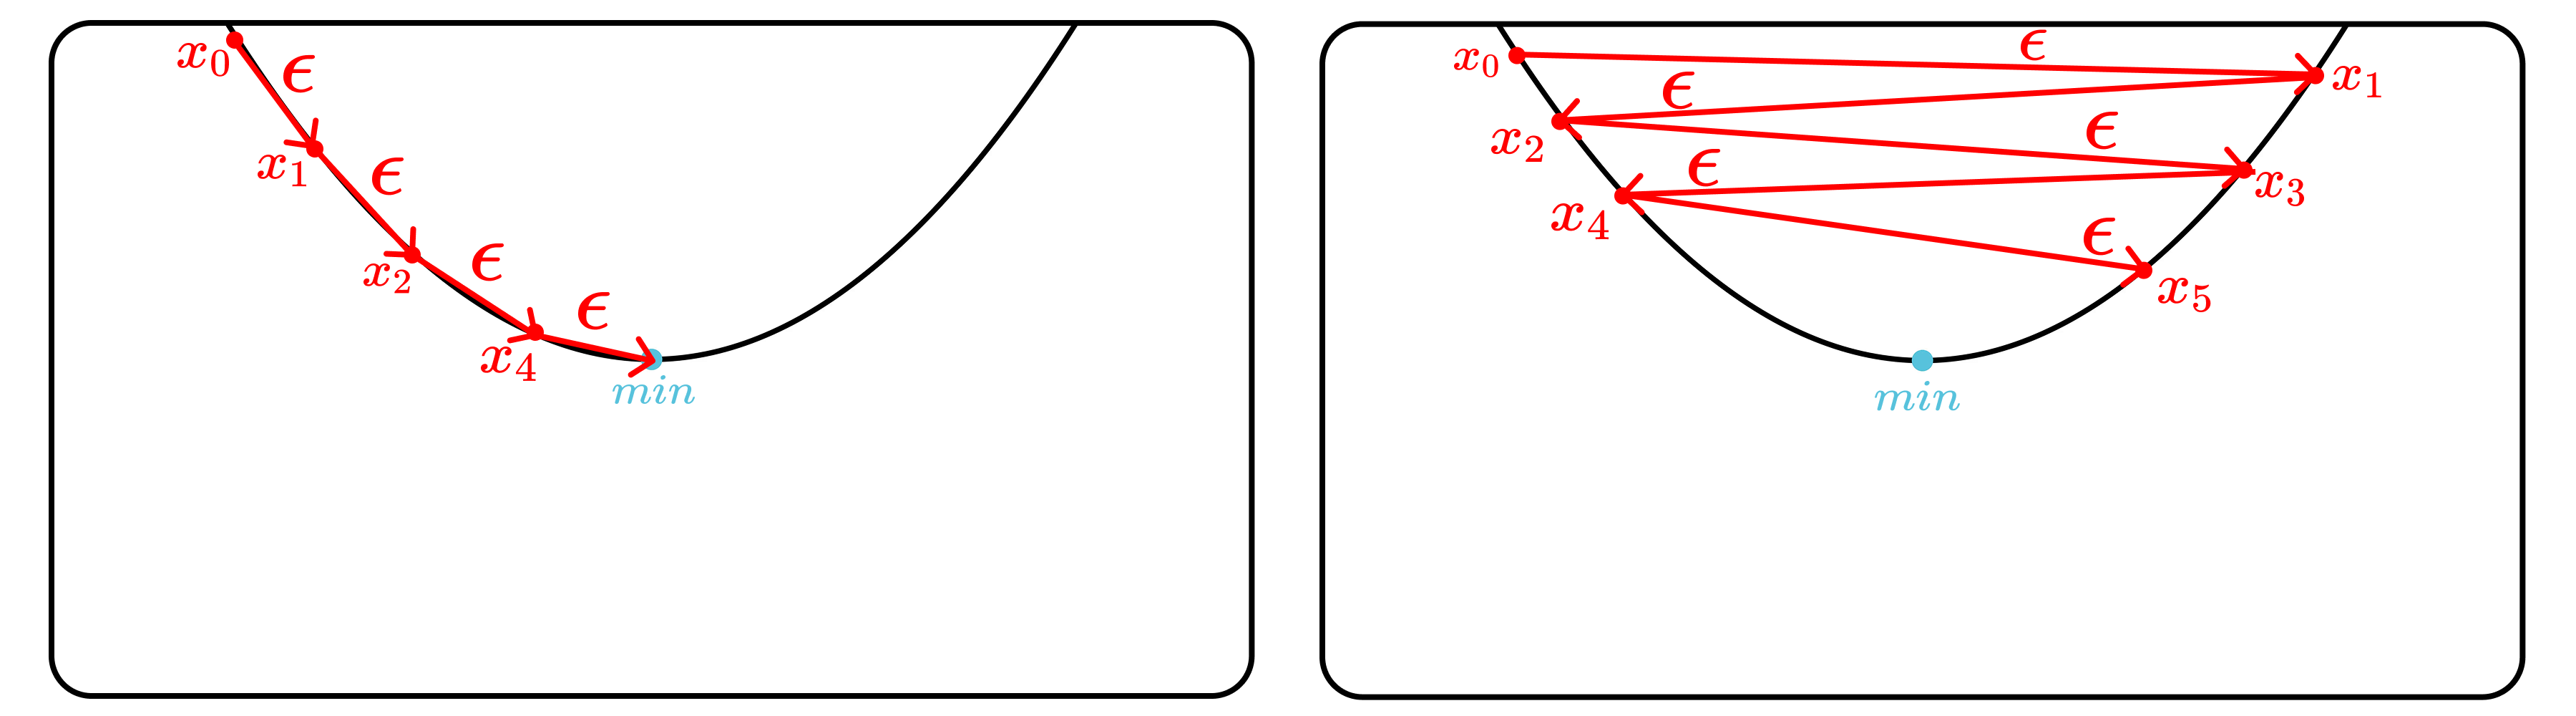
\includegraphics[width=1\linewidth]{../imagens/retropropagacao-gradiente/comparativo-de-passos.png}
    \caption{Comparativo do tamanho de passos em uma função polinomial.}
    \label{fig:comparativo-tamanho-do-passo}
    \fonte{O autor (2025).}
\end{figure}

Na prática, escolher o valor da taxa de aprendizado é uma tarefa que irá depender de modelo em modelo, também irá variar com os diferentes métodos de otimização além da topologia da rede neural que está sendo construída. É sempre recomendado então experimentar diferentes tamanhos de passo, de forma que seja encontrado um que melhor se ajusta ao cenário que está sendo trabalhado.

Outro ponto que deve-se atentar é com relação as funções que estão sendo analisadas ao utilizar o método do gradiente mas também qualquer otimizador que seja baseado nele. Caso tenha uma função convexa (como a representada na ilustração da esquerda da Figura \ref{fig:funcao-convexa-nao-convexa}), em que seu formato lembra um funil, será bem mais fácil para o modelo encontrar o ponto de mínimo global daquela função. Mas se essa função for uma função não convexa (como a representada na ilustração da direita da Figura \ref{fig:funcao-convexa-nao-convexa}), cheia de ondas e com muitos pontos de mínimos locais e pontos de sela, a convergência do modelo será pior, pois existe a chance de que ele fique preso em um ponto de mínimo local ou em um ponto de sela. Isso irá afetar diretamente o desempenho da rede neural que estará sendo criada, fazendo com que ela tenha métricas piores. O problema é que muitas das vezes a função $f(x)$ que estaremos interessados para calcular o desemepenho do modelo será não convexa, dificultando o seu aprendizado.

\begin{figure}[h!]
\centering

% --- Gráfico 1: Função 3D Convexa ---
\begin{minipage}{0.48\textwidth}
    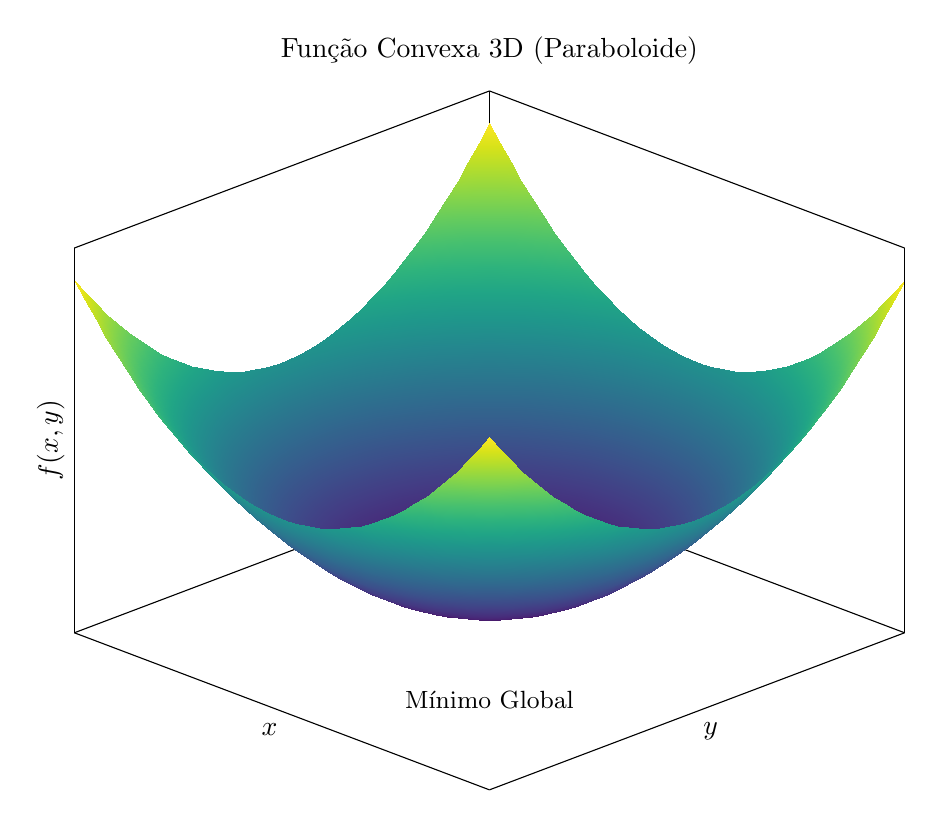
\begin{tikzpicture}
        \begin{axis}[
            title={Função Convexa 3D (Paraboloide)},
            xlabel=$x$,
            ylabel=$y$,
            zlabel={$f(x,y)$},
            xtick=\empty, ytick=\empty, ztick=\empty, % Remove marcações
            view={45}{30}, % Define o ângulo de visão 3D
            width=\textwidth,
            colormap/viridis, % Define o esquema de cores
        ]
        
        % Plot da superfície 3D z = x^2 + y^2
        \addplot3[
            surf, % Tipo de gráfico: superfície
            shader=interp, % Cores interpoladas para um visual suave
            domain=-2:2,
            domain y=-2:2,
            samples=40, % "Resolução" da malha
        ] {x^2 + y^2};
        
        % Marcador para o mínimo global
        \node at (axis cs:0,0,-2) [below, font=\small] {Mínimo Global};
        
        \end{axis}
        \label{fig:funcao-convexa}
    \end{tikzpicture}
\end{minipage}
\hfill % Espaço entre as figuras
% --- Gráfico 2: Função 3D Não-Convexa ---
\begin{minipage}{0.48\textwidth}
    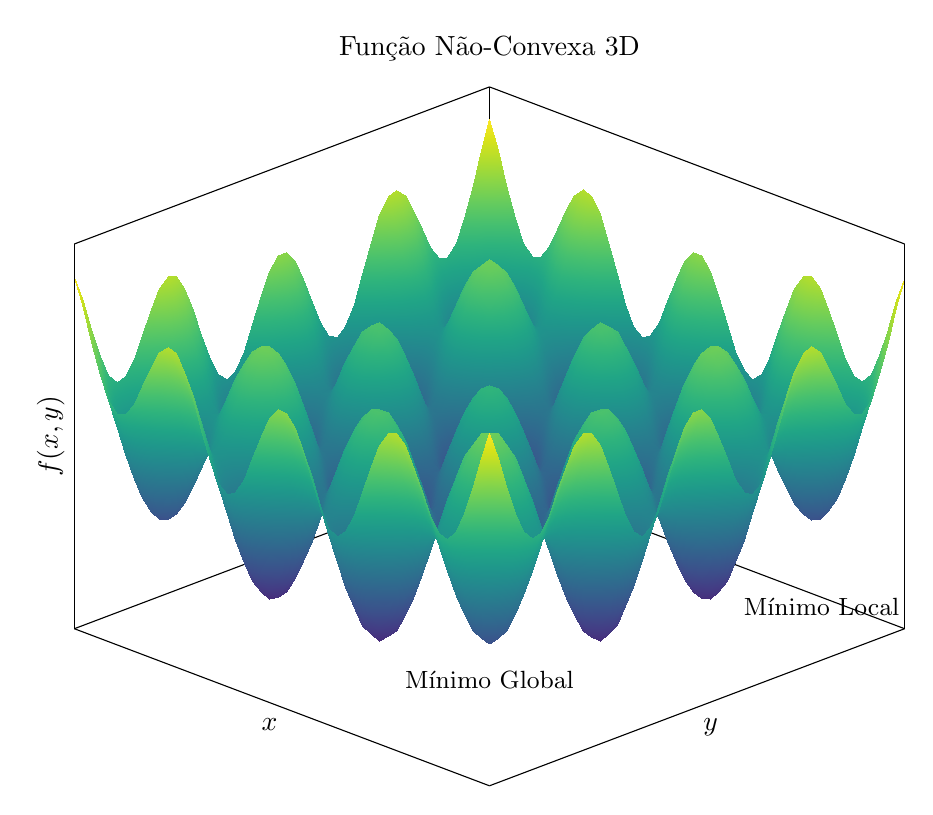
\begin{tikzpicture}
        \begin{axis}[
            title={Função Não-Convexa 3D},
            xlabel=$x$,
            ylabel=$y$,
            zlabel={$f(x,y)$},
            xtick=\empty, ytick=\empty, ztick=\empty,
            view={45}{30},
            width=\textwidth,
            colormap/viridis,
        ]
        
        % Plot da superfície com "ondinhas"
        % A função é um paraboloide + cossenos para criar as ondas
        \addplot3[
            surf,
            shader=interp,
            domain=-2.5:2.5,
            domain y=-2.5:2.5,
            samples=50,
        ] {(x^2+y^2)/5 + 2 - cos(deg(180*x)) - cos(deg(180*y))};
        
        % Marcadores para os mínimos
        \node at (axis cs:0,0,-1) [below, font=\small] {Mínimo Global};
        \node at (axis cs:2,2,0) [font=\small] {Mínimo Local};
        
        \end{axis}
        \label{fig-funcao-nao-convexa}
    \end{tikzpicture}
\end{minipage}
\caption{Comparação entre funções 3D convexas e não-convexas.}
\label{fig:funcao-convexa-nao-convexa}
\fonte{O autor (2025).}
\end{figure}

Além de ser representado utilizando equações, o método do gradiente pode ser expresso também utilizando pseudocódigo para escrever o Algortimo \ref{alg:metodo-do-gradiente}. Perceba que ele recebe como parâmetros de entrada uma taxa de aprendizado $\eta$, o vetor contendo os parâmetros iniciais $\theta_t$ e uma função de perda $f(\theta)$ a ser otimizada.

\begin{algorithm}[H] % A opção [H] tenta colocar o algoritmo exatamente aqui
    \caption{O Método do Gradiente}
    \label{alg:metodo-do-gradiente}
    \begin{algorithmic}[1] % O [1] habilita a numeração das linhas

    \Require Taxa de aprendizado $\eta$
    \Require Vetor de parâmetros inicial $\theta_0$
    \Require Função a ser otimizada $f(\theta)$

    \While{não convergir}
        \State $\textbf{g}_t \leftarrow \nabla_{\theta_{t-1}} f(\theta_{t-1})$
        \State $\theta_t \leftarrow \theta_{t-1} - \eta \textbf{g}_t$
    \EndWhile

    \State \Return $\theta_t$ \Comment{Parâmetros resultantes}
    \end{algorithmic}
\end{algorithm}

Conhecendo o funcionamento do método do gradiente, é possível agora entender a retropropagação, e como ela utiliza esse método para otimizar os pesos das redes neurais garantindo assim um aprendizado eficiente e também a automatização das trocas de parâmetros presentes em uma rede neural.

% ===================================================================
% A Retropropagação
% ===================================================================

\section{A Retropropagação: Aprendendo com os Erros} \index{Retropropagação}

Ainda no contexto de utilizar com o vetor gradiente para otimizar um modelo de rede neural, existe uma ferramenta que trabalha justamente com essse processo, ela é a \gls{retropapagacao} ou \textit{backpropagation} em inglês.

\begin{definicaomoderna}{\textbf{Definição:}}
A \textbf{retropropagação} é uma ferramenta que veio para permitir que redes que fazem o uso de unidades de neurônios possam aprender, para isso, o procedimento ajusta repetidamente os pesos das conexões da rede para minimizar a diferença entre o valor atual da saída do vetor da rede neural com o valor real desejado \parencite{BackpropagationArticle}.
\end{definicaomoderna}

Essa ferramenta foi introduzida para a comunidade científica pelos pesquisadores \textcite{BackpropagationArticle} no texto \textit{Learning Representations by Back-Propagating Errors}, e será explicada nessa seção de forma detalhada. Para isso os autores comecam introduzindo três diferentes funções que serão utilizadas ao longo do texto para deduzir o os conceitos da retropropagação do gradiente, sendo elas: a equação do neurônio, a função de ativação sigmoide e a função de custo do erro quadrático médio \parencite{BackpropagationArticle}.

A primeira função, representada na Equação \ref{eq:neuronio-camada-densa}, explica como um neurônio de uma camada densa irá funcionar quando recebe determinadas entradas \footnote{Caso você leitor decida olhar o artigo original, verá que os autores utilizaram notações diferentes na fórmula do neurônio, eles utilizam algo na forma $x_i = \sum_i y_i \cdot w_{ji}$, sem o viés, mas na prática, eles adicionam o viés como um peso extra que terá valor fixo igual a 1, na prática, ele pode ser tratado com um peso normal, por isso a notação mais simplificada \parencite{BackpropagationArticle}.}.

\begin{equation}
    x_j = (\sum_i y_i \cdot w_{ji}) + b_j
    \label{eq:neuronio-camada-densa}
\end{equation}

Sendo que:

\begin{itemize}
    \item $x_j$: representa a saída de um neurônio $j$;
    \item $y_i$: representa a entrada do neurônio $j$, a qual é resultado da saída de um neurônio $i$ da camada anterior;
    \item $w_{ji}$: representa o peso da conexão entre o neurônio $i$ com o neurônio $j$;
    \item $b_j$: representa o viés do neurônio $j$.
\end{itemize}

A segunda fórmula diz respeito a função de ativação que será utilizada, neste caso, \textcite{BackpropagationArticle} utilizam a sigmoide logísitca, representada na Equação \ref{eq:retropropagacao-sigmoide}, mas eles explicam que essa função pode variar conforme o problema, porém recomendam ter uma derivada limitada além de ser não linear, para que o modelo possa aprender de forma mais efciente.

\begin{equation}
    y_j = \sigma(x_j) = \frac{1}{1 + e^{-x_j}}
    \label{eq:retropropagacao-sigmoide}
\end{equation}

Assim, a sigmoide é a função que irá transformar a saída do neurônio $x_j$ em uma saída $y_j$ que vai ser passada para o neurônio da camada seguinte. Além das duas notações da equação do neurônio, existe uma terceira, que já imbute a função de ativação na equação do neurônio, nesse livro, utilizaremos uma implementação de camadas, em que elas não possuem a função embutida, assim, caso decida que a saída da camada densa deva passar por uma função de ativação, ela deverá ser passada como uma camada separada, sendo algo da forma: camada densa, seguida de camada de ativação.

Por fim, a última equação que os autores discutem para entender a retropropagação é a da função de custo, ou também chamada de erro. No texto, os autores utilizam a função do erro quadrático médio (\textit{MSE}) \parencite{BackpropagationArticle}. A qual calcula o erro entre a saída atual do modelo e o valor real desejado, depois ela eleva ao quadrado esse valor, e por último, divide pela metade. Ela é dada pela Equação \ref{eq:retropropagacao-mse}.

\begin{equation}
    E = \frac{1}{2} \sum_{c} \sum_{j} (y_{j, c} - d_{j, c})^2 
    \label{eq:retropropagacao-mse}
\end{equation}

Em que:

\begin{itemize}
    \item $E$: representa o valor do erro;
    \item $y_{j, c}$: representa o valor atual da saída do neurônio $j$ para o caso $c$;
    \item $d_{j, c}$: representa o valor desejado para o neurônio $j$ para o caso $c$
\end{itemize}

Considerando essas equações, \textcite{BackpropagationArticle} explicam que o objetivo é reduzir o valor do erro $E$, para isso, eles aplicam o método do gradiente para encontrar o ponto de mínimo da função \textit{MSE}. De forma que o primeiro passo é diferenciar o valor da função de erro em relação a cada um dos pesos da rede neural, assim, deve-se calcular $\partial E / \partial y_k$ para um caso específico $k$, e depois generalizar a situação. Com isso, é possível encontrar uma expressão da forma:

\[
    \frac{\partial E}{\partial y_k} = \frac{\partial}{\partial y_k} \left[ \frac{1}{2} \sum_c \sum_k (y_{k, c} - d_{j, c})^2\right]
\]

O primeiro passo é suprimir a soma sobre os casos $c$, pois, consideramos apenas de um caso específico $k$, então a expressão se simplifica para:

\[
    \frac{\partial E}{\partial y_k} = \frac{\partial}{\partial y_k} \left[ \frac{1}{2} \sum_k (y_{k, c} - d_{j, c})^2\right]
\]

A próxima etapa é abrir a soma, para isso, será considerado que existem $n$ neurônios na camada, assim, a expressão fica:

\[
    \frac{\partial E}{\partial y_k} = \frac{\partial}{\partial y_k} \left[ \frac{1}{2} \left( (y_1 - d_1)^2 + (y_2 - d_2)^2 + \cdots (y_k - d_k)^2 + \cdots + (y_n - d_n)^2 \right) \right]
\]

Note que todos os termos que não possuem o índice $k$, como a parte $(y_1 - d_1)^2$, serão valores constantes, e portanto, a sua derivada será igual a zero. Com base nisso, é possível obter uma versão ainda mais simplificada, sendo ela:

\[
    \frac{\partial E}{\partial y_k} = \frac{\partial}{\partial y_k} \left[ \frac{1}{2} (y_k - d_k)^2 \right]
\]

Agora, o último passo é aplicar a regra da cadeia na expressão que sobrou para poder calcular a derivada, neste caso, será considerado que $u = (y_k - d_k)$, assim a expressão final fica:

\[
    \frac{\partial E}{\partial y_k} = \frac{1}{2} \cdot 2u \cdot \frac{\partial u}{\partial y_k} = (y_k - d_k) \cdot 1 = (y_k - d_k)
\]

Voltando para o índice $j$ da notação inicial, é possível concluir que o gradiente do erro (para a função MSE) em relação a uma saída específica de um neurônio é dado pela diferença da saída da unidade pela resultado desejado, ou seja:

\[
    \frac{\partial E}{\partial y_j} = (y_j - d_j) 
\]

O próximo passo proposto pelos autores, consiste em calcular o gradiente do erro em relação a entrada do neurônio $j$, para entender como o erro total muda em relação a uma variação na entrada do neurônio. Para isso, é preciso encontrar então a expressão $\partial E / \partial x_j$ \parencite{BackpropagationArticle}.

Assim, a primeira etapa é aplicar a regra da cadeia, pois, como a entrada do neurônio $x_j$ não aparece diretamente na equação do erro. Então, utilizando essa técnica, é possível derivar o erro em relação a saída do neurônio $y_j$ e multiplicá-lo pela derivada da saída do neurônio em relação a sua entrada. Com base nisso, a expressão inicial é:

\[
    \frac{\partial E}{\partial x_j} = \frac{\partial E}{\partial y_j} \cdot \frac{\partial y_j}{\partial x_j}
\]

Perceba duas coisas nessa expressão, a primeira é que o primeiro termo é resultamente o primeiro, $\partial E / \partial y_j$ que foi calculado e desenvolvido na expressão na primeira parte dessa demonstração, de forma que é possível substituir esse termo na expressão por $y_j - d_j$. A segunda informação, é de que o termo $\partial y_i / \partial x_j$ é justamente a derivada da função de ativação em relação a sua entrada, ou seja, $\sigma'(x_j)$, assim, a derivada da sigmoide será dada por:

\[
    \frac{d y_i}{d x_j} = y_j (1 - y_j)
\]

Sendo assim, a expressão final fica:

\begin{equation}
     \frac{\partial E}{\partial x_j} = \frac{\partial E}{\partial y_j} \cdot y_j \cdot (1 - y_j)
     \label{eq:gradiento-do-erro-em-relacao-a-entrada-de-um-neuronio-para-a-mse-e-sigmoide}
\end{equation}

Note que é possível generalizar essa expressão, dessa forma o gradiente do erro da entrada de um neurônio é o gradiente do erro da saída do neurônio multiplicado pela derivada da função de ativação $\sigma'$ em relação a sua entrada $x_j$.

\begin{equacaodestaque}{Cálculo do Gradiente do Erro em Relação à Entrada de um Neurônio}
    \frac{\partial E}{\partial x_j} = \frac{\partial E}{\partial y_j} \cdot \sigma'(x_j)
    \label{eq:gradiente-do-erro-em-relacao-a-entrada-de-um-neuronio}
\end{equacaodestaque}

Em que:

\begin{itemize}
    \item $\partial E / \partial x_j$: Representa como o erro varia em relação à uma entrada $x_j$ de um neurônio $j$;
    \item $\partial E / \partial y_j$: Representa como o erro varia em relação à uma saída de uma função de ativação que recebe a saída do neurônio $j$;
    \item $\sigma'(x_j)$: Representa a derivada da função de ativação calculada para os valores de $x_j$.
\end{itemize}

Note que $\sigma'(x_j)$ representa a derivada de uma função de ativação qualquer, neste caso representa a sigmoide logística. Mas pode ser outra função, como a tangente hiperbólica ou a \textit{ReLU}. Um ponto importante a ser destacado, é que como a retropropagação trabalha com o método do gradiente, as derivadas são parte essencial do algoritmo, utilizar funções de ativação que possuem derivadas complexas, ou que não podem ser derivadas em grande parte do seu domínio, acabam por dificultar o algortimo. Caso a função possua uma derivada complexa, o cálculo do gradiente irá demorar mais, pois levará uma quantidade maior de operações para computar o valor da derivada.

O próximo passo vai mais além ainda, agora, como \textcite{BackpropagationArticle} explicam, o seu objetivo é entender como o gradiente muda em relação à um peso $w_{ji}$ específico da rede neural, para isso, é preciso calcular a expressão $\partial E / \partial w_{ji}$. Note mais uma vez que o peso $w_{ji}$ não aparece diretamente na equação do erro, de forma que é necessário mais uma vez aplicar a regra da cadeia para calcular essa derivada. Assim, a expressão inicial é:

\[
    \frac{\partial E}{\partial w_{ji}} = \frac{\partial E}{\partial x_j} \cdot \frac{\partial x_j}{\partial w_{ji}}
\]

Note que o primeiro termo da expressão é justamente o que foi calculado na Equação \ref{eq:gradiente-do-erro-em-relacao-a-entrada-de-um-neuronio}, portanto, é preciso calcular apenas o segundo termo, $\partial x_i / \partial w_{ji}$, ou seja, a derivada da entrada do do neurônio em relação a um peso específico. Obtendo então a expressão incial:

\[
    \frac{\partial x_j}{\partial w_{ji}} = \frac{\partial}{\partial w_{ji}} \left[ \left( \sum_i y_i \cdot w_{ji} \right) + b_j\right]
\]

Perceba que o viés, dado por $b_j$ é uma constante, e por isso, não depende do peso $w_{ji}$, então a sua derivada será igual a zero, isso nos permite simplicar a expressão para:

\[
    \frac{\partial x_j}{\partial w_{ji}} = \frac{\partial}{\partial w_{ji}} \left[\sum_i y_i \cdot w_{ji}\right]
\]

Em seguida, é possível abrir a soma, encontrando os termos:

\[
    \frac{\partial x_j}{\partial w_{ji}} = \frac{\partial}{\partial w_{ji}} \left[ (y_1 \cdot w_{j1}) + (y_2 \cdot w_{j2}) + \cdots (y_i \cdot w_{ji}) + \cdots (y_n \cdot w_{jn})\right]
\]

Veja que para qualquer termo que o índice não é $w_{ji}$ a derivada será igual a zero, pois eles serão constantes em relação ao peso $w_{ji}$, dessa forma, é possível simplificar mais uma vez a expressão obtendo:


\[
    \frac{\partial x_j}{\partial w_{ji}} = \frac{\partial}{\partial w_{ji}} \left[  y_i \cdot w_{ji} \right]
\]

Como $y_i$ é uma constante em relação a $w_{ji}$ a derivada final será dada por:

\[
    \frac{\partial x_j}{\partial w_{ji}} = y_i
\]

Agora é possível voltar para a expressão inicial, obtendo então a expressão final para o gradiente do erro em relação a um peso específico da rede neural, sendo ela dada então pelas equações \ref{eq:gradiente-do-erro-em-relacao-a-um-peso-de-um-neuronio}

\begin{equacaodestaque}{Cálculo do Gradiente do Erro em Relação a um Peso de um Neurônio}
    \frac{\partial E}{\partial w_{ji}} = \frac{\partial E}{\partial x_j} \cdot y_i \quad \text{ou} \quad \frac{\partial E}{\partial w_{ji}} = \frac{\partial E}{\partial y_j} \cdot \sigma'(x_j) \cdot y_i
    \label{eq:gradiente-do-erro-em-relacao-a-um-peso-de-um-neuronio}
\end{equacaodestaque}

Em que: 

\begin{itemize}
    \item $\partial E / \partial w_{ji}$: Representa como o erro varia em relação à variação de um peso $w_{ji}$, responsável por conectar os neurônios das camadas $i$ e $j$;
    \item $\partial E / \partial x_j$: Representa como o erro varia em relação à uma entrada do de um neurônio $j$;
    \item $y_i$: Representa a saída da função de ativação de um neurônio da camada $i$;
    \item $\partial E / \partial y_j$: Representa como o erro varia em relação à saída de uma função de ativação de um neurônio $j$;
    \item $\sigma'(x_j)$: Representa a derivada da função de ativação calculada para os valores do neurônio $x_j$.
\end{itemize}

Dessa forma, é possível concluir que o gradiente do erro em relação a um peso específico de um neurônio é dado pelo gradiente do erro da saída do neurônio multiplicado pela derivada da função de ativação em relação a sua entrada e, por fim, multiplicado pela entrada do neurônio.

O próximo passo não está no artigo original, ele envolve entender como o erro varia em relação a um viés de um neurônio específico, ou seja, é preciso calcular a expressão $\partial E / \partial b_j$. Note que mais uma vez o viés $b_j$ não aparece diretamente na equação do erro, ele está dentro da equação do neurônio, assim, novamente é preciso aplicar a regra da cadeia para encontrar essa derivada. Com isso, a expressão inicial é dada por:

\[
    \frac{\partial E}{\partial b_j} = \frac{\partial E}{\partial x_j} \cdot \frac{\partial x_j}{\partial b_j}
\]

O primeiro termo, $\partial E / \partial x_j$, já foi calculado na Equação \ref{eq:gradiente-do-erro-em-relacao-a-entrada-de-um-neuronio}, assim, é preciso focar apenas na segunda parte da expressão, $\partial x_j / \partial b_j$, que é responsável por avaliar como a saída do neurônio $x_j$ varia em relação ao viés $b_j$. Com base, nisso, é possível chegar na expressão:

\[
    \frac{\partial E}{\partial b_j} = \frac{\partial}{\partial b_j} \left[ \left( \sum_k y_k \cdot w{jk} \right) + b_j \right]
\]

Note que os termos que não possuem o viés, como a parte que faz a soma da multiplicação das entradas pelos pesos, $\sum_k y_k \cdot w_{jk}$, são constantes em relação ao viés, portanto, a sua derivada será igual a zero, de tal forma que é possível simplificar a expressão para:

\[
        \frac{\partial E}{\partial b_j} = \frac{\partial}{\partial b_j} \left[ b_j \right]
\]

Com base nessa expressão, é possível concluir que a derivada da saída do neurônio em relação ao viés é igual a 1. Assim, voltando para a expressão inicial, temos que o gradiente do erro em relação ao viés de um neurônio específico é dado pelo gradiente do erro da entrada entrada total desse neurônio, ou seja, a Equação \ref{eq:gradiente-do-erro-em-relacao-a-um-vies-de-um-neuronio}.

\begin{equacaodestaque}{Cálculo do Gradiente do Erro em Relação a um Viés de um Neurônio}
    \frac{\partial E}{\partial b_j} = \frac{\partial E}{\partial x_j} \quad \text{ou} \quad \frac{\partial E}{\partial b_j} = \frac{\partial E}{\partial y_j} \cdot \sigma'(x_j)
    \label{eq:gradiente-do-erro-em-relacao-a-um-vies-de-um-neuronio}
\end{equacaodestaque}

Em que:

\begin{itemize}
    \item $\partial E / \partial b_j$: Representa como o erro varia em relação ao viés $j$;
    \item $\partial E / \partial x_j$: Representa como erro varia em relação à entrada $x_j$ do neurônio $j$;
    \item $\partial E / \partial y_j$: Representa como erro varia em relação à saída da função de ativação que recebe as saídas do neurônio $j$;
    \item $\sigma'(x_j)$: Representa a derivada da função de ativação calculada para os valores de $x_j$.
\end{itemize}

\subsection{Utilizando o Gradiente Descendente para Atualizar os Pesos e Vieses}

Já que é possível calcular o gradiente do erro em relação a um peso específico de um neurônio, e também em relação a um viés específico de um neurônio, o próximo passo proposto pelos autores é utilizar o método do gradiente como uma forma de atualizar os pesos (e também os vieses no nosso caso) da rede neural, de forma a minimizar o valor do erro com pequenas atualizações em cada um desses parâmetros \parencite{BackpropagationArticle}.

Note que o método do gradiente, explicado na seção anterior diz que para atualizar um parâmetros, é preciso pegar o valor atual do parâmetro, e subtrair dele o valor do gradiente multiplicado pelo tamanho do passo (ou taxa de aprendizado). Dessa forma, a regra de atualização para um peso específico é dada pela Equação \ref{eq:regra-de-atualizacao-de-um-peso-atraves-do-metodo-do-gradiente}


\begin{equacaodestaque}{Regra de Atualização de um Peso Através do Método do Gradiente}
    w_{t+1} = w_{t} - \eta \frac{\partial E}{\partial w}
    \label{eq:regra-de-atualizacao-de-um-peso-atraves-do-metodo-do-gradiente}
\end{equacaodestaque}

Em que:

\begin{itemize}
    \item $w_{t+1}$ representa o valor do peso atualizado após o incremento do método do gradiente;
    \item $w_t$ representa o valor inicial do peso na iteração $t$;
    \item $\eta$ representa o tamanho do passo / taxa de aprendizado;
    \item $\partial E / \partial w$ representa o gradiente do erro em relação ao peso.
\end{itemize}

Analogamente, a regra de atualização de um viés pelo método do gradiente é dada pela Equação \ref{eq:regra-de-atualizacao-de-um-vies-atraves-do-metodo-do-gradiente}

\begin{equacaodestaque}{Regra de Atualização de um Viés Através do Método do Gradiente}
    b_{j, t+1} = b_{j, t} - \eta \frac{\partial E}{\partial b_j}
    \label{eq:regra-de-atualizacao-de-um-vies-atraves-do-metodo-do-gradiente}
\end{equacaodestaque}

\begin{itemize}
    \item $b_{j, t+1}$ representa o viés $b_j$ atualizado após o incremento do gradiente;
    \item $b_{j, t}$ representa o valor inicial do viés $b_j$ na iteração $t$;
    \item $\eta$ representa o tamanho do passo / taxa de aprendizado;
    \item $\partial E / \partial b_j$ representa o gradiente do erro em relação ao viés.
\end{itemize}

Um ponto a ser destacado, é que quando estiver trabalhando com uma camada densa de neurônios, você não irá lidar com um neurônio específico, e sim como uma conjunto inteiro deles. Dessa forma, eles estrão distribuidos de forma vetorizada, que que terá um vetor de vieses, uma matriz de pesos e um vetor de neurônios. Assim, as Equações \ref{eq:regra-de-atualizacao-do-vetor-de-pesos-atraves-do-metodo-do-gradiente} e \ref{eq:regra-de-atualizacao-do-vetor-de-vieses-atraves-do-metodo-do-gradiente}, resumem as regras de atualização de pesos e vieses, respectivamente, para casos em que estiver lidando com um conjunto de vetores ao invés de somente um dado.

\begin{equacaodestaque}{Regra de Atualização do Vetor de Pesos Através do Método do Gradiente}
    \mathbf{w}_{t+1} = \mathbf{w}_t - \eta \nabla_{\mathbf{w}} E
    \label{eq:regra-de-atualizacao-do-vetor-de-pesos-atraves-do-metodo-do-gradiente}
\end{equacaodestaque}

Em que: 

\begin{itemize}
    \item $\textbf{w}_{t+1}$: Representa a matriz de pesos atualizada após o incremento do método;
    \item $\textbf{w}_{t}$: Representa a matriz de pesos no instânte atual $t$;
    \item $\eta$: Representa a taxa de aprendizado;
    \item $\nabla_{\textbf{w}} E$: Representa o vetor gradiente do erro calculado em relação aos pesos.
\end{itemize}

\begin{equacaodestaque}{Regra de Atualização do Vetor de Vieses Através do Método do Gradiente}
    \mathbf{b}_{t+1} = \mathbf{b}_t - \eta \nabla_{\mathbf{b}} E
    \label{eq:regra-de-atualizacao-do-vetor-de-vieses-atraves-do-metodo-do-gradiente}
\end{equacaodestaque}

Em que: 

\begin{itemize}
    \item $\textbf{b}_{t+1}$: Representa o vetor de vieses atualizado após o incremento do método;
    \item $\textbf{b}_{t}$: Representa o vetor de vieses no instânte atual $t$;
    \item $\eta$: Representa a taxa de aprendizado;
    \item $\nabla_{\textbf{b}} E$: Representa o vetor gradiente do erro calculado em relação aos vieses.
\end{itemize}

\subsection{Entendendo Como o Gradiente É Propagado ao Longo de Muitas Camadas}

Por fim, com base no que foi explicado até agora, é possível entender melhor como o gradiente passa de uma acamada para a outra durante a retropropagação, para isso será analisada um rede com quatro camadas densas, sendo elas:

\begin{itemize}
    \item \textbf{Camada 1 (Entrada):} Ela possui neurônios com o indice $i$;
    \item \textbf{Camada 2 (Oculta 1):} Ela possui neurônios com o indice $j$;
    \item \textbf{Camada 3 (Oculta 3):} Ela possui neurônios com o indice $k$;
    \item \textbf{Camada 4 (Oculta 3):} Ela possui neurônios com o indice $l$;
\end{itemize}

O objetivo é calcular o gradiente de um peso da primeira camada de pesos, $w_{ji}$, ou seja, é um peso que conecta um neurônio da camada $i$ com um neurônio da camada $j$. Assim, o primeiro passo é utilizar a fórmula \ref{eq:gradiente-do-erro-em-relacao-a-um-peso-de-um-neuronio}, que calcula o gradiente do erro em relação a um peso quaquer.

\[
    \frac{\partial E}{\partial w_{ji}} = \frac{\partial E}{\partial x_j} \cdot y_i
\]

Para encontrar esse gradiente, é preciso desenvolver a expressão $\partial E / \partial x_j$, que representa o gradiente do erro da entrada de um neurônio $j$ da primeira camada oculta. Para isso, é possível utilizar como base a Equação \ref{eq:gradiente-do-erro-em-relacao-a-entrada-de-um-neuronio}, obtendo então:

\[
    \frac{\partial E}{\partial x_j} = \frac{\partial E}{\partial y_j} \cdot \sigma'(x_j)
\]

Nessa expressão, $\sigma'(x_j)$ representa a função de ativação, já o termo $\partial E / \partial y_j$ representa o gradiente que está vindo da camada de cima, a camada $j$, o qual será dado por:

\[
    \frac{\partial E}{\partial x_j} = \sum_k \frac{\partial E}{\partial x_k} \cdot w_{kj}
\]

Juntando os dois termos:

\[
    \frac{\partial E}{\partial x_j} = \left( \sum_k \frac{\partial E}{\partial x_k} \cdot w_{kj} \right) \sigma'(x_j)
\]

Agora, é preciso calcular o termo $\partial E / \partial x_k$, de forma que será possível trazer o gradiente da camada de saída $l$, assim temos:

\[
    \frac{\partial E}{\partial x_k} = \left( \sum_k \frac{\partial E}{\partial x_l} \cdot w_{lk} \right) \cdot \sigma'(x_k)
\]

Em que $\partial E / \partial x_l$ representa o primeiro gradiente, ele é calculado na camada de saída.

Por último, é preciso combinar essas expressões, encontrando como resultado a expressão:

\[
    \frac{\partial E}{\partial w_{ji}} = \left( \sum_k \left[ \left( \sum_l \frac{\partial E}{\partial x_l} \cdot w_{lk} \right) \sigma'(x_k) \right] \cdot w_{kj} \right) \sigma(x_j) \cdot y_i
\]

Com base nessa expressão, é possível concluir que o gradiente de uma camada inicial é proporcional a uma cadeia de multiplicações dos pesos e das derivadas das funções de ativação das camadas posteriores, de forma que é possível simplificar isso para:

\[
    \frac{\partial E}{\partial w_{\text{primeira camada}}} \propto (\text{gradiente da saída}) \cdot (w_{\text{camada 3}} \cdot \sigma'_{\text{camada 3}}) \cdot (w_{\text{camada 2}} \cdot \sigma'_{\text{camada 2}})
\]

Generalizando essa expressão, é possível concluir que o gradiente para uma camada é dado ela Equação \ref{eq:gradiente-para-n-camadas}.

\begin{equacaodestaque}{Gradiente para N Camadas}
    \delta^{(L)} = \left( \left( \textbf{W}^{(L+1)} \right)^T \delta^{(L+1)} \right)  \odot \sigma'(x^{(L)})
    \label{eq:gradiente-para-n-camadas}
\end{equacaodestaque}

Em que: 

\begin{itemize}
    \item $L$: Representa o índice de uma camada, podendo ser um valor entre $1$ (indicando que é uma camada de entrada) ou $n$ (indicando que é uma camada de saída);
    \item $\textbf{W}^{(L)}$: Representa a matriz dde pesos que conecta a camada $L - 1$ à camada $L$;
    \item $b^{(L)}$: Representa o vetor de viés da camada $L$;
    \item $x^{(L)}$: Representa o vetor de entradas totais para os neurônios da camada $L$ antes da ativação;
    \item $y^{(L)}$: Representa o vetor de saídas da camada $L$
    \item $\delta^{(L)}$: Representa o vetor do gradienye na camada $L$;
    \item $\sigma'(x^{(L)})$: Representa o vetor contendo a derivada da função de ativação para cada neurônio da camada $L$;
    \item $\odot$: O produto de Hadamard, que significa multiplicação elemento a elemento.
\end{itemize}

Assim, com base na Equação \ref{eq:gradiente-para-n-camadas}, é possível compreender como o gradiente irá se propagar ao longo de uma rede neural. Esse é um dos pontos mais importantes, pois, qualquer alteração que mude o fluxo do gradiente em uma rede irá afetar diretamente o treinamento da mesma. Existem certos tipos de função de ativação que afetam diretamente como o gradiente é passado de camada em camada, fazendo com que ao ser propagado pelo \textit{backward pass}, tenha seu valor reduzido consideravelmente, tornando um problema para as primeiras camadas da rede, as quais irão receber um gradiente muito pequeno e com isso as atualizações dos pesos e vieses serão mínimas, e com isso a rede sofra para aprender características mais básicas. 

Além disso, existem outras funções de ativação que possuem o efeito inverso, fazendo com que o gradiente "exploda", atrapalhando diretamente como os pesos e vieses serão atualizados no aprendizado da rede.

Para isso, o Capítulo \ref{cap:ativacao-sigmoidais} foca em entender as pricipais funções sigmoidais, como a sigmoide e a tangente hiperbólica, e como essas possuem uma forte relação com o problema do desaparecimento de gradientes. Em seguida, o Capítulo \ref{cap:ativacao-retificadoras} busca introduzir as funções retificadoras, como a \textit{ReLU}, e como elas podem ser uma alternativa para contornar esse problema. Contudo, isso não as torna perfeitas, elas ainda são suceptíveis à outro tipo de problema: a explosão de gradientes; e, no caso da \textit{ReLU}: o problema dos \textit{ReLUs} agonizantes.

Conhecendo como a retropropagação funciona é possível se aprofundar ainda mais em diferentes otimizadores baseados no gradiente. Os quais possuem a mesma ideia de utilizar o vetor gradiente como uma "bússola" indicando os pontos de mínimo da função, porém neste caso, esses outros métodos buscam acelerar o processo de otimização, garantindo uma quantidade menor de iterações para encontrar o mínimos.

% ===================================================================
% Otimizadores Baseados em Gradiente
% ===================================================================

\section{Otimizadores Baseados em Gradiente: Melhorando o Gradiente Descendente}

Como \textcite{BackpropagationArticle} explicam logo ao terminar a dedução do cálculo da atualização dos pesos utilizando o método do gradiente, esse processo pode ser bastante lento quando comparado com métodos que fazem uso de derivadas de segunda ordem, que certamente são mais caras para serem implementadas no computador. Assim, os autores recomendam uma variação do método do gradiente que faz uso de momento com intuito de acelerar a convergência a um custo computacional menor que o de implementar derivadas de segunda ordem \parencite{BackpropagationArticle}.

Além disso, foram surgindo também outras variantes do método do gradiente, como a sua versão estocástica, trazendo uma natureza aleatória para as iterações do método, bem como o gradiente em \textit{mini-batch}, que permite separar os parâmetros do modelo em lotes, podendo ser treinados de forma incremental. Uma outra variante é o gradiente acelerado de Nesterov, ele se diferencia dos outros otimizadores por adicionar o conceito de "\textit{lookahead}", servindo de inspiração para uma variante do \textit{Adam}, um dos algoritmos de otimização modernos.

Assim, essa seção busca introduzir esses novos métodos, de forma que sejam destacadas as suas diferenças ao método do gradiente tradicional, bem como quais as melhorias eles apresentam. Primeiro será visto o gradiente com momento.

\subsection{Método do Gradiente com Momento} \index{Otimizadores!Método do Gradiente com Momento}

Uma boa analogia para entender como o método do gradiente com momento funciona é pensar é uma pedra rolando morro abaixo. No começo, quando ela não havia pegado muita velocidade, ela demorava para rolar e dependendo podia quase parar em algum pedaço do morro, mas conforme foi descendo, foi ganhando mais velocidade, de forma que quando chegar no final do morro, a sua velocidade será bem maior do que quando estava no topo do mesmo. Essa variante funciona de forma parecida com a pedra rolando morro abaixo.

Da mesma forma que o método do gradiente não surgiu originalmente no contexto do aprendizado de máquina, a sua variante com momento não foi diferente. Um os artigos que trabalha com esse conceito de utilizar o momento para acelerar a velocidade do método do gradiente e com isso obter uma convergência mais rápida é o \textit{Some methods of speeding up the convergence of iteration methods}, do pesquisador da URSS \textcite{polyak1964}, nele o autor busca criar métodos iterativos mais rápidos para resolver equações funcionais. Para isso, ele introduz um método de "dois passos", que consiste na junção do método do gradiente com um segundo termo que dá inércia ao método, por último, ele justifica que esse método trás de fato uma convergência mais veloz quando comparado com métodos como o do gradiente.

O método do gradiente com momento de Polyak pode ser visto na Equação \ref{eq:metodo-do-gradiente-com-momentum-de-polyak}.

\begin{equacaodestaque}{Método do Gradiente com Momentum de Polyak}
        \theta_{t+1} = \theta_t - \eta \nabla f(\theta_t) + \beta(\theta_t - \theta_{t-1})
    \label{eq:metodo-do-gradiente-com-momentum-de-polyak}
\end{equacaodestaque}

Em que:

\begin{itemize}
    \item $\theta_{t+1}$: Representa as coordenadas do ponto após a iteração do método;
    \item $\theta_t$: Representa as coordenadas do ponto na iteração $n$;
    \item $\eta$: Representa a taxa de aprendizado / tamanho do passo
    \item $\beta$: Representa a "inércia", controlando a influência do passo anterior no passo atual;
    \item $\theta_{t-1}$: Representa as coordenadas do ponto na iteração anterior.
\end{itemize}

Para calcular $\beta$, \textcite{polyak1964} determina que será utilizada a expressão:

\[
    \beta = \left( \frac{\sqrt{M} - \sqrt{m}}{\sqrt{M} + \sqrt{m}} \right)^2
\]

Em que $M$ representa o maior valor da matriz hessiana, equanto $m$ é o menor valor da matriz hessiana, neste caso, ambos $M$ e $m$ são calculados no ponto de mínimo da função. Isso significa que esses valores não são conhecidos de antemão. Entretanto o maior problema da fórmula proposta por Polyak é que ela exige muitos cálculos, imagine ter que calcular a matriz hessiana de uma função de perda para uma rede que possui milhares ou até milhões de parâmetros, isso é muita coisa e também muito demorado. Assim, no artigo da retropropagação, \textcite{BackpropagationArticle}, apresentam uma fórmula diferente, com intuito dimunuir a quantidade de cálculos a serem feitas, mas mantendo a principal caracterísitca do método do gradiente com momento: a inércia. Ela é dada pela Equação \ref{eq:metodo-do-gradiente-com-momentum-da-retropropagacao}

\begin{equacaodestaque}{Método do Gradiente com Momentum de Rumelhart et. al.}
        \Delta w (t) = \eta \nabla f(x) + \alpha \Delta w(t-1)
    \label{eq:metodo-do-gradiente-com-momentum-da-retropropagacao}
\end{equacaodestaque}

Em que:

\begin{itemize}
    \item $\Delta w(t)$: Representa a variação nos pesos;
    \item $\eta$: Representa a taxa de aprendizado;
    \item $\nabla f(x)$: Representa o gradiente;
    \item $\alpha$: Representa um fator de decaimento exponencial entre 0 e 1 que determina a contribuição do gradiente passado para o gradiente futuro.
\end{itemize}

De forma semelhante ao método do gradiente, o método do gradiente com momento utilizando no artigo da retropropagação também pode ser expresso em forma de pseudocódigo como no Algoritmo \ref{alg:metodo-do-gradiente-com-momento}. Perceba que ele recebe como parâmetros os mesmos do método do gradiente, a taxa de aprendizado $\eta$, o vetor contendo os parâmetros iniciais $\theta_0$, a função de perda $f(\theta)$, mas também recebe o coeficiente de momento $\alpha$. Em seguida, calculá-se o vetor gradiente para o instante $t-1$ e com base nele é feita a atualização do vetor de parâmetros seguindo a Equação \ref{eq:metodo-do-gradiente-com-momentum-da-retropropagacao}.

\begin{algorithm}[H] % A opção [H] tenta colocar o algoritmo exatamente aqui
    \caption{O Método do Gradiente com Momento (versão de \parencite{BackpropagationArticle})}
    \label{alg:metodo-do-gradiente-com-momento}
    \begin{algorithmic}[1] % O [1] habilita a numeração das linhas

    \Require Taxa de aprendizado $\eta$
    \Require Coeficiente de momento $\alpha$
    \Require Vetor de parâmetros inicial $\theta_0$
    \Require Função a ser otimizada $f(\theta)$

    \State $\Delta \theta \gets 0$ \Comment{Inicializa a atualização anterior}

    \While{não convergir}
        \State $\textbf{g}_t \leftarrow \nabla_{\theta_{t-1}} f(\theta_{t-1})$
        \State $\theta_t \leftarrow \theta_{t-1} - \eta \textbf{g}_t + \alpha \Delta \theta$
    \EndWhile

    \State \Return $\theta_t$ \Comment{Parâmetros resultantes}
    \end{algorithmic}
\end{algorithm}

Sabendo o método do gradiente como momento, é possível também conhecer outras soluções que buscam fazer uso do vetor gradiente para encontrar os pontos de mínimo, neste caso, na seção seguinte será analisado o método do gradiente estocástico ou \textit{stochastic gradient descent (SGD)}.

\subsection{Método do Gradiente Estocástico (SGD)} \index{Otimizadores!Método do Gradiente Estocástico (SGD)}

Assim como o método do gradiente que faz uso do momento para acelerar a convergência e com isso diminuir um número de iterações gastas para se encontrar o ponto de mínimo, o método do gradiente estocástico também não surgiu no contexto do aprendizado de máquina. Esse método fez sua primeira aparição no trabalho \textit{A Stochastic Approximation Method}, dos autores \textcite{StochasticGradientDescentMethod}, em que eles introduzem uma forma de encontrar as raízes de uma função quando esta não pode ser observada de forma direta, mas apenas através de medições com ruído.

Contudo, apenas nos anos 60 métodos que se baseiam no cálculo de funções de erro com ruido passaram a aparecer no cenário de aprendizado de máquina, como foi o caso dos pesquisadores \textcite{Adeline} com \textit{ADALINE (Adaptive Linear Neuron)}. Nele, os autores buscam otimizar os valores dos pesos dos neurônios de uma rede em que ao calcular o erro do modelo, este era afetado por ruído \parencite{Adeline}

Conforme o tempo foi passando, o \textit{SGD} provou ser uma excelente alternativa para encontrar pontos de mínimo em uma função de perda quando comparado com o método do gradiente tradicional. Isso se dá ao fato da sua natureza estocástica, que o permite "saltar" por pontos de mínimos locais e também por pontos de sela, contudo, ele pode não garantir uma convergência tão boa quando comparado ao método tradicional, podendo chegar muito próximo do ponto de mínimo, mas escapando dele, devido a suas prioriedades aleatórias \parencite{MaosAObra}.

O \textit{SGD} funciona da seguinte forma: ele seleciona uma instância aleatória do conjunto de treinamento a cada etapa, e com base nessa instância, ele calcula o gradiente \parencite{MaosAObra}. De tal forma que de um lado existe o gradiente descendente vetorizado, que foi visto nas Equações \ref{eq:regra-de-atualizacao-do-vetor-de-pesos-atraves-do-metodo-do-gradiente} (para a regra de atualização de um vetor de pesos) e \ref{eq:regra-de-atualizacao-do-vetor-de-vieses-atraves-do-metodo-do-gradiente} (para a regra de atualização de um vetor de vises), fazendo as atualizações em todos os parâmetros de uma vez só, enquanto de de outro lado existe o método do gradiente estocástico que utiliza apenas um parâmetro por vez. O SGD certamente será mais rápido, pois precisa que menos parâmetros estejam na memória principal para que as atualizações possam ser feitas, mas por outro lado acaba adicionando aleatoriedade para o processo de otimização.

\begin{equacaodestaque}{Método do Gradiente Estocástico (SGD)}
    \theta_{t+1} = \theta_t - \eta \nabla_{\theta} J(\theta; x^{(i)}, y^{(i)})
    \label{eq:metodo-do-gradiente-estocastico}
\end{equacaodestaque}

Em que:

\begin{itemize}
    \item $\theta_{t+1}$: representa o vetor de parâmetros do modelo após a atualização (na iteração $t+1$).
    \item $\theta_t$: representa o vetor de parâmetros do modelo na iteração atual $t$.
    \item $\eta$: representa a taxa de aprendizado.
    \item $\nabla_{\theta} J(\theta; x^{(i)}, y^{(i)})$: representa o gradiente da função de custo $J$ em relação aos parâmetros $\theta$. É calculado utilizando apenas uma única amostra $(x^{(i)}, y^{(i)})$ do conjunto de dados.
\end{itemize}

Por ser um método que depende da aleatoriedade para calcular os parâmetros a serem atualizados, o \textit{SGD} possui um comportamento mais imprevisível. Como pode ser visto na Figura \ref{fig:comparativo-gd-sgd}, enquanto o gradiente em \textit{batch} segue um caminho suave encontrar o ponto de mínimo global, o gradiente estocástico segue uma trajetória irregular, justamente pelo fato de não considerar todos os parâmetros de uma vez. Na prática, isso pode acabar afetando o desempenho do \textit{SGD}, o qual irá demorar mais para convergir, contudo, ele acaba compensando essa demora ao ser mais rápido para calcular as iterações do método.

\begin{figure}[h!]
    \centering
    \begin{tikzpicture}[font=\small]
        \begin{axis}[
            title={Comparativo de Trajetórias de Otimização},
            xlabel={Parâmetro $\theta_1$},
            ylabel={Parâmetro $\theta_2$},
            % --- ADICIONE ESTAS LINHAS PARA DEFINIR O TAMANHO DO GRÁFICO ---
            xmin=-5.5, xmax=5.5,
            ymin=-5.5, ymax=5.5,
            % --- FIM DAS LINHAS ADICIONADAS ---
            view={0}{90},
            enlargelimits=false,
            axis lines=none,
            width=12cm,
            height=10cm,
            clip=false
        ]

        % --- MUDANÇA PRINCIPAL AQUI ---
        % 1. Plot das curvas de nível (função de custo)
        % O bloco \addplot3 foi removido e substituído pelas elipses manuais abaixo.
        % Usamos (axis cs:0,0) para centralizar as elipses no gráfico.
        % Os raios foram ajustados para conterem todo o desenho.
        \draw[gray!30] (axis cs:0,0) ellipse (5 and 4.8);
        \draw[gray!50] (axis cs:0,0) ellipse (4 and 3.5);
        \draw[gray!70] (axis cs:0,0) ellipse (3 and 2.2);
        \draw[gray!85] (axis cs:0,0) ellipse (2 and 1.2);
        
        % 2. Ponto de Mínimo Global
        \node[circle, fill=cyan, inner sep=1.5pt, label={[label distance=-0.2cm]270:Mínimo Global}] at (axis cs:0,0) {};

        % 3. Ponto de Início
        \node[circle, fill=black, inner sep=1.5pt] at (axis cs:-3.5, 4.5) {};
        
        % 4. Caminho do Gradiente em Batch (suave)
        \draw[-{Stealth[length=2mm]}, red, thick, line cap=round] (axis cs:-3.5, 4.5)
            to[out=-70, in=150] (axis cs:-0.8, 1)
            to[out=-30, in=120] (axis cs:0.1, 0.1);

        % 5. Caminho do Gradiente Estocástico (ruidoso)
        \draw[-{Stealth[length=2mm]}, blue, thick, line cap=round,
            decorate, decoration={
                random steps,
                segment length=6pt,
                amplitude=3pt
            }
        ] (axis cs:-3.5, 4.5) -- (axis cs:-2.8, 3) -- (axis cs:-3.2, 2) -- (axis cs:-2, 2.5) -- (axis cs:-1.5, 1.2) -- (axis cs:-1.8, 0.5) -- (axis cs:-0.7, 1) -- (axis cs:-0.4, 0.2) -- (axis cs:0.4, 0.6) -- (axis cs:-0.1, 0.1);

        % 6. Legendas para os caminhos
        \node[red, anchor=south west] at (axis cs:-3.5, 4.6) {\textbf{Gradiente em Batch}};
        \node[blue, anchor=west] at (axis cs:-1.5, 3.5) {\textbf{Gradiente Estocástico (SGD)}};

        \end{axis}
    \end{tikzpicture}
    \caption{Comparação visual entre a trajetória suave do Gradiente em Batch e a trajetória ruidosa do Gradiente Estocástico (SGD) para encontrar o mínimo de uma função de custo.}
    \label{fig:comparativo-gd-sgd}
    \fonte{O autor (2025).}
\end{figure}

\subsection{Método do Gradiente em Mini-Batch (GD mini-batch)} \index{Otimizadores!Método do Gradiente em Mini-Batch (GD mini-batch)}

Entendendo como funciona o \textit{SGD}, o próximo passo é conhecer o método do gradiente em \textit{mini-batch}, que busca ser uma alternativa entre o gradiente estocástico e o gradiente em \textit{batch}. Como explica \textcite{MaosAObra}, o \textit{GD mini-batch} calcula os gradientes para pequenos conjuntos aleatórios, chamados \textit{mini-batches}, que fazem parte do conjunto total de parâmetros.

Por utilizar mais parâmetros de uma vez para calcular o gradiente, o gradiente em \textit{mini-batch} possui uma vantagem quando comparado com o gradiente estocástico, ele irá apresentar um progresso de parâmetros menos irregular \parencite{MaosAObra}. Dessa forma, o gradiente em \textit{mini-batch} consegue chegar um pouco mais perto dos pontos de mínimo, ajudando na convergência.

Uma boa vantagem do \textit{GD mini-batch} está no fato que esses \textit{batches} podem ter tamanhos escolhidos pelo programador, de forma que caso a máquina que esteja usando possua uma quantidade maior de memória \textit{ram}, você pode utilizar \textit{batches} maiores, ajudando na convergência do modelo para melhores pontos de mínimo.

\subsection{Gradiente Acelerado de Nesterov (NAG)} \index{Otimizadores!Gradiente Acelerado de Nesterov (NAG)}

Uma outra variante do método do gradiente é o gradiente acelerado de Nesterov (\textit{NAG}). Ele foi introduzido no artigo \textit{A method for solving the convex programming problem with convergence rate $O(1/k^2)$} do autor \textcite{NAGMethod}, em que é apresentado como uma forma computacionamente mais barata de resolver problemas de programação convexa. 

No texto, o autor trás a adição de um novo conceito para encontrar os pontos de mínimos, o chamado ponto de \textit{lookahead} (olhar para frente em português), o qual serve de base para os cálculos do gradiente \parencite{NAGMethod}. Assim o \textit{NAG} possui dois passos: o primeiro consiste no cálculo da predição futura (no ponto de \textit{lookahead}), dando um passo na direção do momento anterior, em seguida, com base nesse novo ponto calculado, é possível encontrar o valor do gradiente e com isso, atualizar os parâmetros da rede neural.

A sua expressão é mostrada na Equação \ref{eq:gradiente-acelerado-de-nesterov}.

\begin{equacaodestaque}{Gradiente Acelerado de Nesterov (NAG)}
    \begin{aligned}
        \theta_{\text{lookahead}} &= \theta_t + \beta(\theta_t - \theta_{t-1}) \\
        \theta_{t+1} &= \theta_{\text{lookahead}} - \eta \nabla_{\theta} J(\theta_{\text{lookahead}}) 
    \end{aligned}
    \label{eq:gradiente-acelerado-de-nesterov}
\end{equacaodestaque}

Em que:

\begin{itemize}
    \item $\theta_{\text{lookahead}}$: Representa a posição futura estimada, que serve como ponto de "lookahead".
    \item $\theta_{t+1}$: Representa o vetor de parâmetros atualizado após o passo de otimização.
    \item $\theta_t$: Representa o vetor de parâmetros na iteração atual.
    \item $\theta_{t-1}$: Representa o vetor de parâmetros da iteração anterior, usado para calcular o momento.
    \item $\beta$: Representa o coeficiente de momento.
    \item $\eta$: Representa a taxa de aprendizado.
    \item $\nabla_{\theta} J(\theta_{\text{lookahead}})$: Representa o gradiente da função de custo $J$.
\end{itemize}

Note, que o \textit{NAG} é também uma variante do método do gradiente que faz uso do momento ou inércia para atualizar os parâmetros do modelo que está sendo treinado. Essa ideia de utilizar o momento como facilitador, permitindo encontrar pontos de mínimo de forma mais rápida, é utilizada até hoje em alguns otimizadores, o \textit{NAdam}, uma variante do otimizador \textit{Adam}, busca justamente implementar conceitos do gradiente acelerado de Nesterov no \textit{Adam} e com isso conseguir alcançar convergências mais rápidas.

Para melhor entender o funcionamento do ponto de \textit{lookahead} do \textit{NAG}, é possível visualizar a Figura \ref{fig:funcionamento-nag}. Perceba que primeiro o modelo dá um passo em direção ao \textit{lookahead} utilizando o momento, em seguida, é feita a correção da direção utilizando como base o vetor gradiente. Dessa forma, o gradiente acelerado de Nesterov, ao utilizar o momento, consegue acelerar a convergência e com isso, encontrar pontos de mínimo mais rapidamente.

\begin{figure}[h!]
    \centering
    \begin{tikzpicture}[
        >={Stealth[length=2.5mm, width=2mm]},
        point/.style={circle, fill=black, inner sep=1.3pt},
        font=\small
    ]
        % --- Fundo: Curvas de Nível ---
        \draw[gray!30] (0,0) ellipse (4.5 and 3);
        \draw[gray!50] (0,0) ellipse (3.5 and 2.2);
        \draw[gray!70] (0,0) ellipse (2.5 and 1.5);

        % --- Coordenadas dos Pontos ---
        \coordinate (theta_t) at (-3.5, 2.0);
        \coordinate (lookahead) at (-1.0, 0.9);
        \coordinate (theta_t_plus_1) at (0.2, -0.3);

        % --- Vetores e Descrições ---
        % 1. Vetor do momento (passo de lookahead)
        \draw[->, blue, very thick] (theta_t) -- (lookahead);

        % 2. Vetor do gradiente (calculado no ponto de lookahead)
        \draw[->, red, very thick] (lookahead) -- (theta_t_plus_1);

        % 3. Vetor da atualização final (para clareza)
        \draw[->, black, thick, dashed] (theta_t) -- (theta_t_plus_1);

        % --- Nós dos Pontos ---
        % (Não adicionei os nós de texto dos vetores para manter o código igual ao seu)
        \node[point, label={[label distance=-1mm]above:$\theta_t$}] at (theta_t) {};
        \node[point, label={[label distance=1mm]right:$\theta_{lookahead}$}] at (lookahead) {};
        \node[point, label={[label distance=-1mm]below:$\theta_{t+1}$}] at (theta_t_plus_1) {};

    \end{tikzpicture}
    \caption{Representação visual do funcionamento do gradiente acelerado de Nesterov. Em azul está representado o primeiro passo em direção ao ponto de \textit{lookahead} utilizando o momento. Em vermelho está o segundo passo, com a atualização utilizando o vetor gradiente para corrigir a direção.}
    \label{fig:funcionamento-nag}
    \fonte{O autor (2025).}
\end{figure}

Sabendo o funcionamento do \textit{NAG}, também é possível desenvolver o seu pseudocódigo como no Algoritmo \ref{alg:nag}. Ele irá receber como entradas uma taxa de aprendizado $\eta$, o coefiente de momento $\mu$, o vetor contendo os parâmetros inicias $\theta_0$ e a função a ser otimizada $f(\theta)$. Com base nisso, se inicia o loop do gradiente acelerado de Nesterov, que começa calculando o vetor gradiente no ponto de \textit{lookahead}, que é seguido da atualização dos parâmetros $\textbf{m}_t$ os quais são utilizandos para fazer a atualização do vetor de parâmetros $\theta$. Dessa forma, o loop termina após convergir para o ponto de mínimo, ou até atingir um número máximo de iterações.

\begin{algorithm}[H] % A opção [H] tenta colocar o algoritmo exatamente aqui
    \caption{Gradiente Acelerado de Nesterov (\textit{NAG})}
    \label{alg:nag}
    \begin{algorithmic}[1] % O [1] habilita a numeração das linhas

    \Require Taxa de aprendizado $\eta$
    \Require Coeficiente de momento $\mu$
    \Require Vetor de parâmetros inicial $\theta_0$
    \Require Função a ser otimizada $f(\theta)$

    \While{não convergir}
        \State $\textbf{g}_t \leftarrow \nabla_{\theta_{t-1}} f(\theta_{t-1} - \eta \mu \textbf{m}_{t-1})$
        \State $\textbf{m}_t \gets \mu \textbf{m}_{t-1} + \textbf{g}_t$
        \State $\theta_t \gets \theta_{t-1} - \eta \textbf{m}_t$
    \EndWhile

    \State \Return $\theta_t$ \Comment{Parâmetros resultantes}
    \end{algorithmic}
\end{algorithm}

\subsection{Comparativo de Otimizadores Clássicos}

Por fim, é possível compilar as características desses otimizadores vistos na Tabela \ref{tab:comparativo-otimizadores-classicos}. Dessa forma, é destacado a principal característica do otimizador, bem como suas vantagens e desvantagens.

\begin{table}[htbp]
    \centering
    \begin{threeparttable}
        \caption{Comparativo de otimizadores clássicos}
        \label{tab:comparativo-otimizadores-classicos}
        % p{3.2cm} define uma largura fixa para a primeira coluna.
        % As 3 colunas 'X' restantes dividem o espaço que sobra de forma flexível.
        % >{\raggedright\arraybackslash} alinha o texto à esquerda para melhor leitura.
        \begin{tabularx}{\textwidth}{p{3.2cm} *{3}{>{\raggedright\arraybackslash}X}}
            \toprule
            \textbf{Otimizador} & \textbf{Característica principal} & \textbf{Vantagem} & \textbf{Desvantagem} \\
            \midrule
            Gradiente descendente (\textit{GD}) & Otimizador clássico que dá origem aos otimizadores baseados em gradiente & Apresenta fácil implementação & Precisa que todo o conjunto de parâmetros esteja na memória para fazer as atualizações e calcular o gradiente. \\
            \addlinespace
            Gradiente descendente estocástico (\textit{SGD}) & Calcula o vetor gradiente para apenas um item do conjunto de parâmetros e faz a atualização. & É mais rápido que o \textit{GD} além de conseguir escapar de pontos de sela e mínimos locais. & Apresenta uma trajetória ruidosa \\
            \addlinespace
            Gradiente descendente em \textit{mini-batch} (\textit{GD mini-batch}) & Calcula o vetor gradiente para pequenos lotes (\textit{batches}) e faz a atualização. & Possui o parámetro tamanho do lote para ser escolhido também. & \\
            \addlinespace
            Gradiente descendente com momento & Faz uso do momento para acelerar a convergência do método. & Consegue encontrar pontos de mínimo mais rapidamente e com menos iterações. & Possui o parâmetro do momento para ser escolhido também \\
            \addlinespace
            Gradiente acelerado de Nesterov (\textit{NAG}) & Faz uso de um ponto de \textit{lookahead} para calcular o vetor gradiente e a partir desse fazer a atualização dos parâmetros & Possui uma convergência mais acelerada que o método tradicional & Apresenta um algoritmo mais custoso para ser implementado. \\
            \bottomrule
        \end{tabularx}
        
        \begin{tablenotes}[para]
            \small
            \item[] Fonte: O autor (2025).
        \end{tablenotes}

    \end{threeparttable}
\end{table}

Visto uma série de otimizadores mais antigos porém muito úteis para a tarefa de encontrar pontos de mínimo, é possível agora discutir os otimizadores mais recentes. Para isso, eles continuam seguindo a mesma ideia, utilizar o vetor gradiente como o parâmetro de indicação para encontrar pontos de mínimo. Porém, fazendo uso de técnicas mais avançadas da matemática e da programação, de forma a garantir não só uma convergência mais rápida, mas também conseguir escapar de pontos de sela e mínimos locais.

\section{Otimizadores Modernos Baseados em Gradiente: A Era das Taxas de Aprendizado Adaptativas}

Conforme os anos foram passando, foram surgindo novos otimizadores, também inspirados em métodos mais clássicos, como o \textit{SGD} e as variantes com momento. Mas, a partir dos anos 2010, uma nova família de otimizadores, que se originou a partir do \textit{AdaGrad}, surgiu. Esses otimizadores tinham a mesma proposta dos outros baseados em gradiente, utilizá-lo como uma bússsola para encontrar os pontos de mínimo, mas ao mesmo tempo apresentavam uma diferença notável quando comparados com os otimizadores clássicos: o uso de diferentes taxas de aprendizado.

Fazer uso de diferentes taxas de aprendizado permitiu que os modelos criados com esses algoritmos apresentassem um desempenho maior. Pois, para caracterísitcas que apareciam menos dos \textit{datasets} era possível atribuir taxas de aprendizados mais altas, como uma forma do modelo prestar mais atenção nessas caracterísitcas. Ao mesmo tempo que atribuir taxas de aprendizado menores para características mais comuns, permitia uma melhor convergência.

\subsection{Adadptive Gradient Algorithm (AdaGrad)} \index{Otimizadores!Adpative Gradient Algorithm (AdaGrad)}

Apresentado para a comunidade científica no texto \textit{Adaptive Subgradient Methods for Online Learning and Stochastic Optimization}, \textit{o Adadptive Gradient Algorithm (AdaGrad)}, foi descrito por \textcite{AdaGradMethod} como uma adpatação dos métodos iterativos baseados em gradiente, que nos permite encontrar "agulhas em palheiros" em forma de características muito preditivas, mas raramente vistas.

O que os autores se referem ao ato de encontrar "agulhas em palheiros", está ligado diretamente na forma como o \textit{AdaGrad} atua para melhorar o desempenho de um modelo tanto para reconhecer caracteríticas que são muito frequentes nos dados de treino quando características que são mais raras. Como \textcite{AdaGradMethod} explicam, esse método faz uso de múltiplas taxas de aprendizado, assim caracterítiscas muito frequentes recebem uma taxa de aprendizado pequena, enquanto caraterísticas menos frequentes recebem uma taxa de aprendizado maior.

Dessa forma, o modelo que está sendo treinado conseque garantir melhores métricas durante o seu aprendizado, pois estará aprendendo sobre aquilo que aparece muito nos dados de treino, mas, quando aparecer algo diferente e menos comum, ele irá "prestar mais atenção" devido à maior taxa de aprendizado nessas características.

O \textit{AdaGrad} veio como uma forma de aplicar técnicas de aprendizado-teórico para problemas online e aprendizado estocástico, focando concretamente no métodos de (sub)gradiente, de forma que a representação desse algoritmo pode ser vista no Algoritmo \ref{alg:adagrad}.

Esse algoritmo recebe como entradas uma taxa de aprendizado $\eta$, o vetor de parâmetros a serem atualizados $\theta_0$, a função a ser otimizada $f(\theta)$, e um parâmetros de estabilidade $\epsilon$, o qual é adicionado no denominador para evitar que divisões por zero ocorram. O primeiro passo feito pelo \textit{AdaGrad} é iniciar um vetor acumulador $\mathbf{n}_0$ que terá a mesma dimensão dos parâmetros $\theta_0$ e será responsável por armazenar a soma dos quadrados dos gradientes passados para cada parâmetro.

Com isso feito, é então iniciado o loop do \textit{AdaGrad}, o qual irá terminar somente quando o modelo convergir. Primeiro, é calculado o vetor gradiente $\textbf{g}_t$ da função de custo $f$ em relação aos parâmetros atuais da rede, como ele é um vetor gradiente, cabe destacar que ele estará apontando para a direção de maior crescimento da mesma função de custo. Em seguida, é calculado o termo $t$ do vetor acumulador $\mathbf{n}_0$, para isso é somado o valor da interação anterior $\textbf{n}_{t-1}$ ao quadrado elemento a elemento do gradiente atual $\textbf{g}_t$. Por fim, o último passo do loop do \textit{AdaGrad} consiste em atualizar os parâmetros do vetor $\theta_t$, para isso é subtraído do parâmetros da iteração anterior $\theta_{t-1}$ a taxa de aprendizado $\eta$ multiplicada pela divisão do vetor acumulador pela raiz quadrada do acumulador $\textbf{n}_t$.

\begin{algorithm}[H] % A opção [H] tenta colocar o algoritmo exatamente aqui
    \caption{AdaGrad}
    \label{alg:adagrad}
    \begin{algorithmic}[1] % O [1] habilita a numeração das linhas

    \Require Taxa de aprendizado $\eta$
    \Require Vetor de parâmetros inicial $\theta_0$
    \Require Função a ser otimizada $f(\theta)$
    \Require Parâmetro de estabilidade $\epsilon$

    \State $\mathbf{n}_0 \leftarrow 0$ \Comment{Inicializar o vetor acumulador}

    \While{não convergir}
        \State $\textbf{g}_t \leftarrow \nabla_{\theta_{t-1}} f(\theta_{t-1})$
        \State $\textbf{n}_t \leftarrow \textbf{n}_{t-1} + \mathbf{g}_t \odot \mathbf{g}_t$
        \State $\theta_t \leftarrow \theta_{t-1} - \eta \frac{\textbf{g}_t}{\sqrt{\textbf{n}_t} + \epsilon}$
    \EndWhile

    \State \Return $\theta_t$ \Comment{Parâmetros resultantes}
    \end{algorithmic}
\end{algorithm}

Note que $\eta$ quando está sendo utilizada para atualizar os parâmetros do modelo, passa a ser divida de elemento a elemento, isso faz com que elementos com um gradiente muito alto, recebam uma taxa de aprendizado baixa, enquando elementos menos comuns, e consequentemente com o gradiente menor, recebam uma taxa de aprendizado mais alta. 

Para comprovar a eficácia do novo algoritmo desenvolvido, \textcite{AdaGradMethod} utilizam uma série de \textit{datasets} a fim de entender melhor em quais cenários, a aplicação do \textit{AdaGrad} pode ser valiosa, para isso, os autores utilizam os \textit{datasets}: \textit{ImageNet} (para classificação de imagens), \textit{MNIST} (para classificação de dígitos manuscritos), o \textit{UCI repository} (para censo de income data), e \textit{Reuters RCV1} (para classificação de textos).

Para a classificação de textos utilizando o \textit{Reuters RCV1}, foram comparados o \textit{AdaGrad-RDA}, o \textit{RDA}, o \textit{FB}, o \textit{AdaGrad-FB}, o \textit{PA} e o \textit{ARROW}; de forma que são analisadas as taxas de erro de cada um desses modelos após o treino, bem como a proporção não-nula, responsável por indicar a quantidade de parâmetros do modelo que são diferentes de zero no final do treinamento, sendo uma medida para avaliar a esparsidade do modelo (quanto menor o número, maior a esparsidade, e potencialmente mais simples é o modelo) \parencite{AdaGradMethod}. Analisando os resultados apresentados por \textcite{AdaGradMethod} é possível ver uma superioridade dos algoritmos \textit{AdaGrad} perante aos outros otimizadores avaliados, além disso, nota-se que o \textit{AdaGrad-RDA} produz modelos mais esparsos quando comparado com a variante \textit{AdaGrad-FB}.

A tabela com as taxas de erro no conjunto de testes para o dataset \textit{Reuters RCV1}, apresentando as métricas encontradas pelos autores pode ser vista na Tabela \ref{tab:resultados-rcv1-adagrad}

\begin{table}[htbp]
    \centering
    \begin{threeparttable} % Inicia o ambiente para a tabela com notas
        \caption{Taxas de erro no conjunto de teste e proporção de não-nulos (entre parênteses) no dataset \textit{Reuters RCV1}}
        \label{tab:resultados-rcv1-adagrad}
        \begin{tabular}{l c c c c c c}
            \toprule
             & RDA & FB & ADAGRAD-RDA & ADAGRAD-FB & PA & AROW \\
            \midrule
            ECAT & .051 (.099) & .058 (.194) & \textbf{.044 (.086)} & \textbf{.044} (.238) & .059 & .049 \\
            CCAT & .064 (.123) & .111 (.226) & \textbf{.053 (.105)} & \textbf{.053} (.276) & .107 & .061 \\
            GCAT & .046 (.092) & .056 (.183) & \textbf{.040 (.080)} & \textbf{.040} (.225) & .066 & .044 \\
            MCAT & .037 (.074) & .056 (.146) & .035 (\textbf{.063}) & \textbf{.034} (.176) & .053 & .039 \\
            \bottomrule
        \end{tabular}
        
        \begin{tablenotes}[para] % Inicia o ambiente das notas
            \small % Define a fonte como menor, padrão ABNT para fontes
            \item[] Fonte: Adaptado de \parencite{AdaGradMethod}.
        \end{tablenotes}

    \end{threeparttable} % Finaliza o ambiente
\end{table}

Já para o \textit{ImageNet}, foram escolhidos apenas 4 algoritmos: o \textit{AdaGrad-RDA}, o \textit{AROW}, o \textit{PA} e o \textit{RDA}, e para avaliar esses otimizadores, foi utilizada como métricas a precisão média (Avg. Prec.), P@K (precisão em k, indicando a porcentagem das vezes em que a resposta correta esteve entre as k primeiras previsões), e também a proporção não-nula \parencite{AdaGradMethod}. Com base nas análises feitas por \textcite{AdaGradMethod}, é possível tirar duas conclusões, a primeira delas é que o \textit{AdaGrad} é o melhor modelo em precisão média além de atingir uma maior esparsidade, contudo o \textit{AROW} ainda é uma melhor alternativa para as precisões em k, o que indica que ele é capaz de atingir as respostas corretas nas primeiras previsões.

Para comparar a precisão dos modelos utilizando o dataset \textit{ImageNet} você pode analisar a Tabela \ref{tab:resultados-imagenet-adagrad}

\begin{table}[htbp]
    \centering
    \begin{threeparttable} % Inicia o ambiente
        \caption{Precisão no conjunto de teste para o \textit{ImageNet}}
        \label{tab:resultados-imagenet-adagrad}
        \begin{tabular}{l c c c c c c}
            \toprule
            Alg. & Avg. Prec. & P@1 & P@3 & P@5 & P@10 & Prop. nonzero \\
            \midrule
            ADAGRAD RDA & \textbf{0.6022} & 0.8502 & 0.8307 & 0.8130 & 0.7811 & \textbf{0.7267} \\
            AROW & 0.5813 & \textbf{0.8597} & \textbf{0.8369} & \textbf{0.8165} & \textbf{0.7816} & 1.0000 \\
            PA & 0.5581 & 0.8455 & 0.8184 & 0.7957 & 0.7576 & 1.0000 \\
            RDA & 0.5042 & 0.7496 & 0.7185 & 0.6950 & 0.6545 & 0.8996 \\
            \bottomrule
        \end{tabular}
        
        \begin{tablenotes}[para] % Ambiente para a fonte
            \small % Define o tamanho da fonte
            \item[] Fonte: Adaptado de \parencite{AdaGradMethod}.
        \end{tablenotes}

    \end{threeparttable} % Finaliza o ambiente
\end{table}

O último comparativo que será visto é com relação ao \textit{MNIST}, nele, \textcite{AdaGradMethod} escolheram cinco algoritmos: o \textit{PA}, o \textit{Ada RDA}, o \textit{RDA}, o \textit{Ada RDA l1/l2} e o \textit{RDA l1/l2}, sendo analisada a quantidade de erros pela quantidade de exemplos vistos. Nessa análise, os algoritmos que performaram melhor foram o PA seguido do Ada RDA, apresentando um comportamento parecido, enquanto isso, nota-se que utilizar as normalizações l1/l2 não trouxeram muitas vantagens para os algoritmos \parencite{AdaGradMethod}.

As curvas de aprendizado dos diferentes modelos treinados pelos autores podem ser vistas na Figura \ref{fig:curvas-de-aprendizado-adagrad-mnist}, note que o \textit{Ada RNA} apresenta uma performance muito parecida com o \textit{PA}, apresentando pouco mais de 5.000 erros ao ser treinado com todo o \textit{dataset}.

\begin{figure}[h]
    \centering
    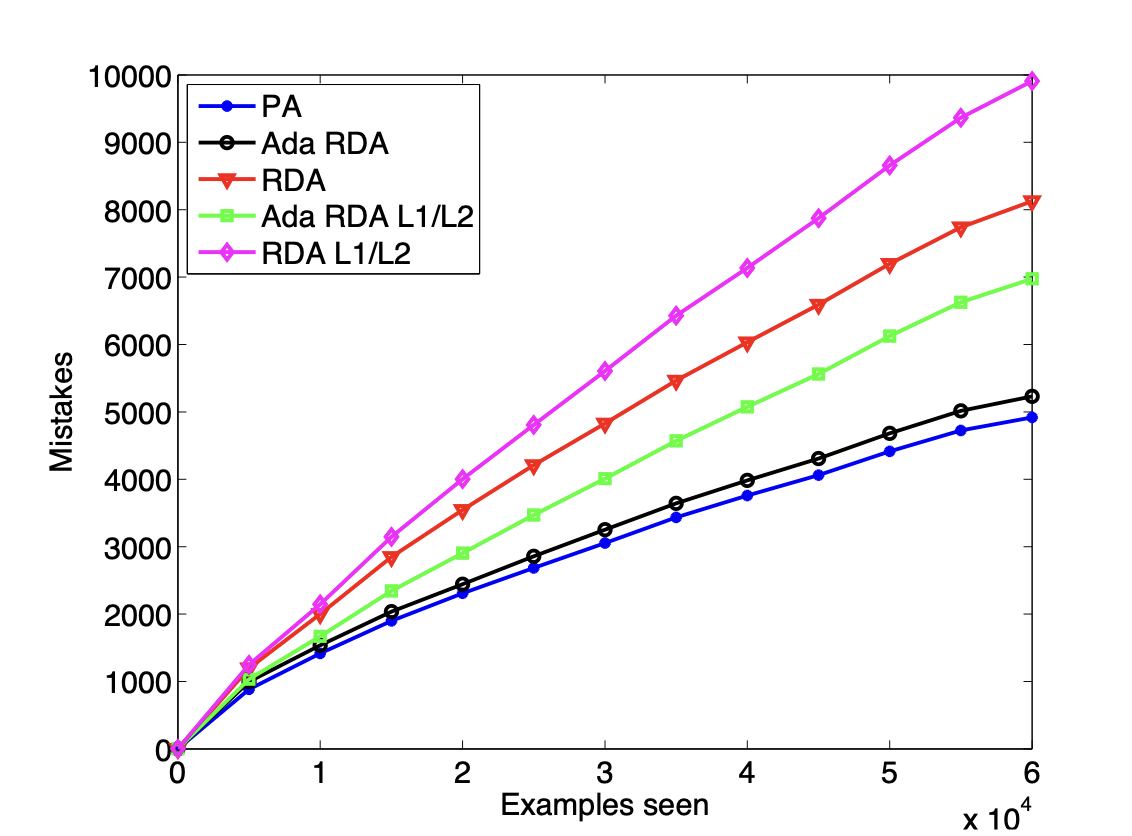
\includegraphics[width=0.65\linewidth]{../imagens/retropropagacao-gradiente/comparativo-adagrad-mnist.png}
    
    \caption[Curvas de aprendizado no MNIST]{%
        Curvas de aprendizado no \textit{dataset} MNIST.
        \newline % Cria uma nova linha para a fonte
        \small Fonte: \parencite{AdaGradMethod}.
    }
    \label{fig:curvas-de-aprendizado-adagrad-mnist}
\end{figure}

\medskip
\begin{center}
 * * *
\end{center}
\medskip

\textbf{Algumas Aplicações do AdaGrad em Otimização de Redes Neurais}
\vspace{1em}

\begin{itemize}
    \item \textbf{Aplicação 1 (Área):}
    \item \textbf{Aplicação 2 (Área):}
    \item \textbf{Aplicação 3 (Área):}
    \item \textbf{Aplicação 4 (Área):}
\end{itemize}

\medskip
\begin{center}
 * * *
\end{center}
\medskip

O \textit{AdaGrad} simbolizou não somente um avanço para os algoritmos de otimização, como também introduziu o conceito de diferentes taxas de aprendizado, permitindo com que um modelo possa aprender bem tanto características muito frequentes como características mais incomuns. Dessa forma, um novo periódo de otimizadores surgiu, seguindo os conceitos do \textit{AdaGrad} mas buscando incrementar o seu algoritmo a fim de corrigir falhas que ficaram para trás. Ao longo dessa seção, serão vistos mais otimizadores que atuam de forma parecida ao \textit{AdaGrad}, adicinando melhorias para o seu desempenho.

\subsection{Root Mean Square Propagation (RMSProp)} \index{Otimizadores!Root Mean Square Propagation (RMSProp)}

Diferente dos outros métodos de otimização que surgiram em artigos, o \textit{RMSProp} tem uma concepação diferente, sendo apresentado por Geoffrey Hinton nas suas notas de aula do curso \textit{Neural Networks for Machine Learning} como um método que semelhante ao AdaGrad, dividia o gradiente \parencite{RMSPropMethod}. Para isso, o \textit{RMSProp} combina a ideia de somente usar o sinal do gradiente com a ideia de adptar o tamanho do passo separadamente para diferentes pesos, de forma que para funcionar em \textit{mini-batches} é mantido uma média móvel do quadrado do gradiente para cada peso \parencite{RMSPropMethod}.

Para inicilizar o \textit{RMSProp} é preciso de cinco parâmetros: a taxa de aprendizado $\eta$, o vetor de parâmetros iniciais $\theta_0$, a função de perda a ser otimizada $f(\theta)$, o parâmetro de estabilidade $\epsilon$, para evitar divisões por zero, e também a taxa de decaimento $\nu$, a qual irá controlar a média móvel dos gradientes. Antes de iniciar o loop do RMSProp é feita a inicialização do vetor acumulador com zeros, ele irá atuar como um acumulador para a média móvel do quadrados dos gradientes.

O primeiro passo ao se iniciar o loop do \textit{RMSProp} é calcular $\textbf{g}_t$, para isso ele irá receber o vetor gradiente da função de custo calculado para os parâmetros da iteração anterior $\theta_{t-1}$, em seguida é atualizado o vetor acumulador da forma que $\textbf{n}_t$ será dado pela multiplicação da taxa de decaimento $\nu$ pelo valor do vetor acumulador na iteração anterior, esse resultado é então somado ao quadrado produto a produto do gradiente $\textbf{g}_t$ multiplicado por $(1 - \nu)$.

O último passo do \textit{RSMProp} consistem em atualizar os parâmetros de $\theta_0$ para isso é subtraído dos parâmetros anteriores $\theta_{t-1}$ a multiplicação da taxa de aprendizado pelo vetor gradiente $\textbf{g}_t$ que é dividido pela raíz do vetor acumulador de parâmetros. Assim, esse loop se repete até atingir o número máximo de épocas escolhido na hora da implementação, ou no caso do pseudocódigo \ref{alg:rmsprop}, ele irá repetir até o modelo convergir, ou seja, quando a norma do vetor gradiente for zero.

\begin{algorithm}[H] % A opção [H] tenta colocar o algoritmo exatamente aqui
    \caption{RMSProp}
    \label{alg:rmsprop}
    \begin{algorithmic}[1] % O [1] habilita a numeração das linhas

    \Require Taxa de aprendizado $\eta$
    \Require Vetor de parâmetros inicial $\theta_0$
    \Require Função a ser otimizada $f(\theta)$
    \Require Parâmetro de estabilidade $\epsilon$
    \Require Taxa de decaimento $\nu$

    \State $\mathbf{n}_0 \leftarrow 0$ \Comment{Inicializar o vetor acumulador}

    \While{não convergir}
        \State $\textbf{g}_t \leftarrow \nabla_{\theta_{t-1}} f(\theta_{t-1})$
        \State $\textbf{n}_t \leftarrow \nu \textbf{n}_{t-1} + (1 - \nu) (\mathbf{g}_t \odot \mathbf{g}_t)$
        \State $\theta_t \leftarrow \theta_{t-1} - \eta \frac{\textbf{g}_t}{\sqrt{\textbf{n}_t} + \epsilon}$
    \EndWhile

    \State \Return $\theta_t$ \Comment{Parâmetros resultantes}
    \end{algorithmic}
\end{algorithm}

Perceba que o \textit{RMSProp} consegue corrigir um dos problemas do \textit{AdaGrad} ao atualizar o vetor acumulador utilizando uma taxa de decaimento $\nu$. No \textit{AdaGrad} o vetor acumalor só cresce, enquanto no RMSProp os termos mais antigos vão tendo seu valor reduzido gradativamente pelo coeficiente $\nu$. Dessa forma, é possível melhor focar nos termos mais recentes que fazem parte do vetor acumulador.

\medskip
\begin{center}
 * * *
\end{center}
\medskip

\textbf{Algumas Aplicações do RMSProp em Otimização de Redes Neurais}
\vspace{1em}

\begin{itemize}
    \item \textbf{Aplicação 1 (Área):}
    \item \textbf{Aplicação 2 (Área):}
    \item \textbf{Aplicação 3 (Área):}
    \item \textbf{Aplicação 4 (Área):}
\end{itemize}

\medskip
\begin{center}
 * * *
\end{center}
\medskip

\subsection{Adaptive Moment Estimation (Adam)} \index{Otimizadores!Adaptive Moment Estimation (Adam)}

Uma evolução natural dos algortitmos de otimização \textit{AdaGrad} e \textit{RMSProp} é o \textit{Adam} ou \textit{Adaptive Moment Estimation}. Esse algortimo foi apresentado pelos pesquisadores \textcite{AdamMethod}, no artigo \textit{Adam: A Method for Stochastic Optimization}, o qual veio para ser um método de otimização estocástica que requere apenas gradientes de primeira ordem com poucos requisitos de memória.

Para isso, o \textit{Adam} computa taxas de aprendizado individuais para diferentes parâmetros para estimações do primeiro e segundo momento do gradiente, de forma que ele é capaz de combinar as vantagens do \textit{AdaGrad}, que trabalha bem com gradientes esparsos, e o \textit{RMSProp}, que trabalha bem \textit{on-line} e em configurações não-estacionárias \parencite{AdamMethod}.

O \textit{Adam} recebe como parâmetros uma taxa de aprendizado $\eta$, os coeficientes de decaimento exponencial $\beta_1$ e $\beta_2$ para as estimativas do momento em um conjunto de intervalos $[0, 1)$. Além disso, recebe também o vetor contendo os parâmetros iniciais $\theta_0$, a função de perda $f(\theta)$ para qual será encontrado o ponto de mínimo, e também o parâmetro de estabilidade $\epsilon$ para evitar divisões por zero.

Com todos esses parâmetros, o primeiro passo consiste em inicializar os vetores de primeiro $\mathbf{m}_0$ e segundo $\mathbf{v}_0$ momento bem como o passo do tempo $t$, para isso, os vetores são zerados e o tempo $t$ também. Feito isso, o loop do Adam se inicia, terminando apenas quando o modelo convergir. Primeiro, é incrementado o tempo, e em seguida calcula-se o gradiente $\mathbf{g}_t$ que irá receber o gradiente da função de perda $f(\theta)$ em relação aos parâmetros da iteração anterior.

A próxima etapa do Adam consiste em atualizar as estimativas des momentos, o primeiro momento $\mathbf{m}_t$ recebe o coeficiente de decaimento $\beta_1$ multiplicado pelo vetor do primeiro momento na iteração anterior, que é então somado a multiplicação de $(1 - \beta_1)$ pelo vetor gradiente $\mathbf{g}_t$. O segundo momento é calculado de forma semelhante, com a diferença de que são utilizados o vetor do segundo momento para fazer as incrementações e o uso do coeficiente $\beta_2$, além disso, na segunda parte da soma é feito o produto termo o termo dos vetores gradientes.

Seguindo adiante, deve-se calcular a correção do viés, para isso $\mathbf{\hat{m}}_t$ irá calcular a divisão do vetor do primeiro momento por $(1 - \beta_1)$, enquanto $\mathbf{\hat{v}}_t$ irá calcular a divisão do vetor do primeiro momento por $(1 - \beta_2)$.

Por fim, é feita a incrementação dos parâmetros de $\theta_0$ de forma semelhante ao \textit{AdaGrad}, eles serão dados pela diferença do vetor de parâmetros na iteração anterior pela multiplicação da taxa de aprendizado $\eta$ com a divisão dos vetores do primeiro e segundo momento.

Esse método pode ser visto no bloco de algoritmo \ref{alg:adam}.

\begin{algorithm}[H]
    \caption{Adaptive Moment Estimation (Adam)}
    \label{alg:adam}
    \begin{algorithmic}[1]

    \Require Taxa de aprendizado $\eta$ (ex: 0.001)
    \Require Coeficientes de decaimento $\beta_1, \beta_2$ (ex: 0.9, 0.999)
    \Require Vetor de parâmetros inicial $\theta_0$
    \Require Função a ser otimizada $f(\theta)$
    \Require Parâmetro de estabilidade $\epsilon$ (ex: 1e-7)

    \State $\mathbf{m}_0 \leftarrow 0$ \Comment{Inicializar vetor de 1º momento (média)}
    \State $\mathbf{v}_0 \leftarrow 0$ \Comment{Inicializar vetor de 2º momento (variância)}
    \State $t \leftarrow 0$ \Comment{Inicializar passo de tempo}

    \While{não convergir}
        \State $t \leftarrow t + 1$
        \State $\mathbf{g}_t \leftarrow \nabla_{\theta_{t-1}} f(\theta_{t-1})$
        
        % Atualiza estimativas dos momentos
        \State $\mathbf{m}_t \leftarrow \beta_1 \mathbf{m}_{t-1} + (1 - \beta_1) \mathbf{g}_t$
        \State $\mathbf{v}_t \leftarrow \beta_2 \mathbf{v}_{t-1} + (1 - \beta_2) (\mathbf{g}_t \odot \mathbf{g}_t)$
        
        % Calcula a correção de viés (bias correction)
        \State $\mathbf{\hat{m}}_t \leftarrow \frac{\mathbf{m}_t}{1 - \beta_1^t}$
        \State $\mathbf{\hat{v}}_t \leftarrow \frac{\mathbf{v}_t}{1 - \beta_2^t}$
        
        % Atualiza os parâmetros
        \State $\theta_t \leftarrow \theta_{t-1} - \eta  \frac{\mathbf{\hat{m}}_t}{\sqrt{\mathbf{\hat{v}}_t} + \epsilon}$
    \EndWhile

    \State \Return $\theta_t$ \Comment{Parâmetros resultantes}
    \end{algorithmic}
\end{algorithm}

Para testar esse novo algoritmo, os pesquisadores \textcite{AdamMethod} prepararam uma série de experimentos, sendo alguns deles envolvendo uma regressão logística, uma rede neural multi-camadas e uma rede convolucional.

No primeiro dos experimentos, os autores avaliam esse otimizador utilizado uma regularização L2 criando uma regressão logística para analisar o \textit{dataset} de dígitos manuscritos \textit{MNIST} \parencite{AdamMethod}. Nos testes, \textcite{AdamMethod} comparam a sua técnica de otimização com o gradiente estocástico acelereado de Nesterov (\textit{SGDNesterov}) e também como o \textit{AdaGrad}; de forma que eles foram capazes de concluir que o \textit{Adam} possui uma convergência similar ao \textit{SGDNesterov}, equanto o \textit{AdaGrad} apresenta uma convergência mais demorada e com um maior custo de treino. Esse compartivo pode ser visto na Figura \ref{fig:comparativo-adam-mnist}.

\begin{figure}[h]
    \centering
    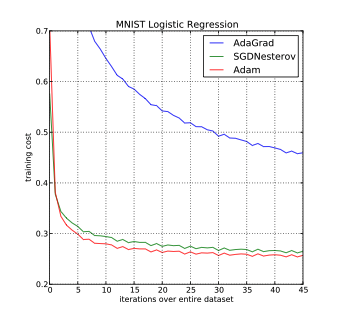
\includegraphics[width=0.65\linewidth]{../imagens/retropropagacao-gradiente/comparativo-adam-mnist.png}
    
    \caption[Curvas de aprendizado no dataset MNIST]{%
        Curvas de aprendizado no dataset MNIST.
        \newline
        \small Fonte: \parencite{AdamMethod}.
    }
    \label{fig:comparativo-adam-mnist}
\end{figure}

No segundo experimento, os cientistas foram capazes de descobrir que mesmo em redes neurais multi-camadas (as quais são modelos com funções objetivas não-convexas), mesmo a análise de convergência feita não se aplicando a problemas não-convexos, o \textit{Adam} foi capaz de performar melhor que outros métodos \parencite{AdamMethod}. Para o teste então, \textcite{AdamMethod} criaram uma rede neural com duas camadas totalmente conectadas com 1000 unidades de neuônio utilizando a função de atiavção \textit{ReLU} com \textit{mini-batch} de tamanho 128, com base nos testes, eles foram capazes de perceber que o \textit{Adam} consegui ser de 5 a 10 vezes mais rápido por iteração que o método \textit{SFO} (\textit{sum-of-functions}), o qual é um método \textit{quasi-Newton} que trabalha também com dados em \textit{mini-batches}. O comportamento desses diferentes otimizadores para uma rede neural multicamadas está retratado nos gráficos da Figura \ref{fig:comparativo-adam-multilayer}.

\begin{figure}[h]
    \centering
    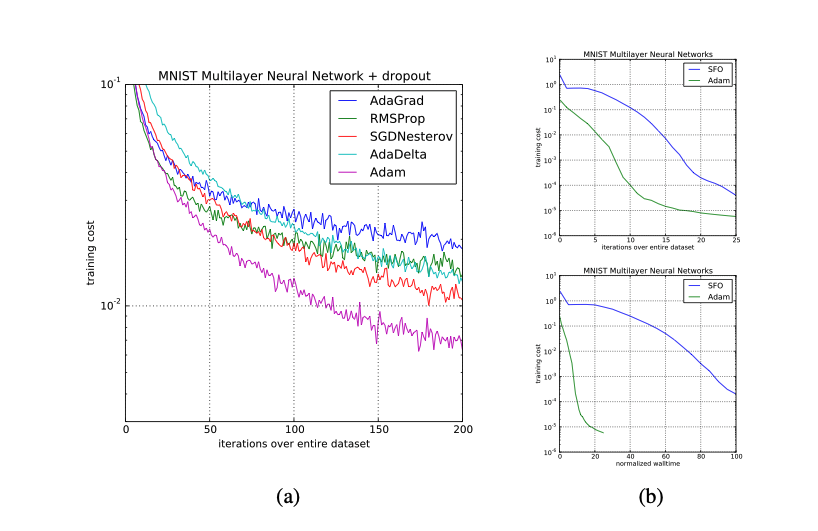
\includegraphics[width=0.85\linewidth]{../imagens/retropropagacao-gradiente/comparativo-adam-multilayer.png}
    
    \caption[Treinamento de redes neurais multicamadas no \textit{MNIST}]{%
        Treinamento de redes neurais multicamadas em imagens \textit{MNIST}. (a) Redes neurais utilizando regularização estocástica com \textit{dropout}. (b) Redes neurais com função de custo determinística, em comparação com o otimizador soma de funções (\textit{SFO}).
        \newline
        \small Fonte: \parencite{AdamMethod}.
    }
    \label{fig:comparativo-adam-multilayer}
\end{figure}

Já para a rede convolucional, \textcite{AdamMethod} criaram uma \textit{CNN} com três camadas, a primeira com filtros de dimensões 5x5, seguida de uma camada de \textit{max pooling} de dimensões 3x3 com \textit{stride} 2 que se liga a uma camada totalmente conectada de 1000 unidades ocultas que faz uso da função de ativação \textit{ReLU}. Com base nas análises, os autores concluíram que tanto o \textit{Adam} quando o \textit{AdaGrad} fazem um progresso rápido no custo inicial do treino, em seguida, o \textit{Adam} e o \textit{SGD} convergem consideravelmente mais rápido que o \textit{AdaGrad} \parencite{AdamMethod}. É possível ver como o \textit{Adam} e os outros otimizadores performam nessa tarefa na Figura \ref{fig:comparativo-adam-convnet}.

\begin{figure}[h]
    \centering
    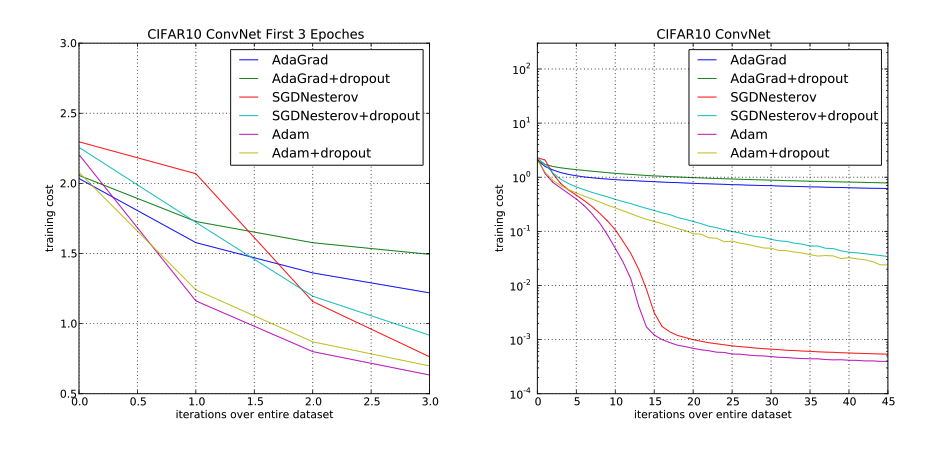
\includegraphics[width=0.85\linewidth]{../imagens/retropropagacao-gradiente/comparativo-adam-convnet.png}
    
    \caption[Custo de treinamento de redes neurais convolucionais]{%
        Custo de treinamento de redes neurais convolucionais. À esquerda, o custo nas três primeiras épocas. À direita, o custo ao longo de 45 épocas.
        \newline
        \small Fonte: \parencite{AdamMethod}.
    }
    \label{fig:comparativo-adam-convnet}
\end{figure}

\medskip
\begin{center}
 * * *
\end{center}
\medskip

\textbf{Algumas Aplicações do Adam em Otimização de Redes Neurais}
\vspace{1em}

\begin{itemize}
    \item \textbf{Aplicação 1 (Área):}
    \item \textbf{Aplicação 2 (Área):}
    \item \textbf{Aplicação 3 (Área):}
    \item \textbf{Aplicação 4 (Área):}
\end{itemize}

\medskip
\begin{center}
 * * *
\end{center}
\medskip

Assim como os métodos \textit{AdaGrad} e \textit{RMSProp} foram grandes inspirações para o desenvolvimento do otimizador \textit{Adam}, é inegável que o mesmo também passou a ser fonte de inspiração para pesquisas futuras, as quais o utilizam como base e faziam pequenos incrementos em seu método a fim de corrigir falhas. Dessa forma, a comunidade científica vive em um constante avanço incremental, pegando as partes boas e de um projeto e melhorando o que pode não estar tão bom. Os próximos otimizadores, são variantes do Adam, de forma que seguem esse mesmo princípio, de pegar algo que estava bom, mas falho em algumas partes e melhorá-lo.

\subsection{AdaMax} \index{Otimizadores!AdaMax}

Ainda em \textit{Adam: A Method for Stochastic Optimization}, os autores \textcite{AdamMethod}, além de apresentarem o \textit{Adam} como um novo otimizador, eles também apresentam uma variante dele, o \textit{AdaMax}, que ao invés de utilizar a norma $L^2$ para calcular o segundo momento, utilizam a norma $L^p$, em que $p \to \infty$, provando ser um algoritmo surpreendemente simples e estável. Dessa forma, os autores foram chegram no otimizador listado no Algortimo \ref{alg:adamax}.

Note que o \textit{AdaMax} recebe como parâmetros de entrada os mesmos parâmetros do \textit{Adam} tradicional, com a diferença sendo na inicilização do vetores, que agora, ao invés de inicilizar o vetor do segundo momento, é inicilizadada a norma infinita $u_0$. No loop do \textit{AdaMax}, é possível ver um funcionamento semelhante ao do Adam, ele começa incrementando o passo de tempo $t$ e e calculando o vetor de gradientes $g_t$ para aquela iteração, que é então utilizado para atualizar o vetor do primeiro momento $m_0$.

A diferença do \textit{AdaMax} está na próxima etapa, em que é atualizada a norma infinita utilizando como base $\max(\beta_2 \cdot u_{t-1}, |g_t|)$. Com base em todos esses parâmetros o \textit{AdaMax} atualiza o vetor de parâmetros $\theta$. Essas iterações são repetidas ate o modelo convergir para um ponto de mínimo.

\begin{algorithm}[H] % A opção [H] tenta colocar o algoritmo exatamente aqui
    \caption{AdaMax, uma variante do Adam baseada na norma infinita}
    \label{alg:adamax}
    \begin{algorithmic}[1] % O [1] habilita a numeração das linhas

    \Require Taxa de aprendizado $\eta$
    \Require Taxas de decaimento exponencial $\beta_1, \beta_2 \in [0, 1)$
    \Require Função objetivo estocástica com parâmetros $\theta$, $f(\theta)$
    \Require Vetor de parâmetros inicial $\theta_0$

    \State $m_0 \leftarrow 0$ \Comment{Inicializar vetor de 1º momento}
    \State $u_0 \leftarrow 0$ \Comment{Inicializar a norma infinita exponencialmente ponderada}
    \State $t \leftarrow 0$ \Comment{Inicializar passo de tempo}

    \While{não convergir}
        \State $t \leftarrow t + 1$
        \State $g_t \leftarrow \nabla_\theta f_t(\theta_{t-1})$ \Comment{Obter gradientes em relação ao objetivo no passo $t$}
        \State $m_t \leftarrow \beta_1 \cdot m_{t-1} + (1 - \beta_1) \cdot g_t$ \Comment{Atualizar estimativa viciada do primeiro momento}
        \State $u_t \leftarrow \max(\beta_2 \cdot u_{t-1}, |g_t|)$ \Comment{Atualizar a norma infinita exponencialmente ponderada}
        \State $\theta_t \leftarrow \theta_{t-1} - (\eta / (1 - \beta_1^t)) \cdot m_t / u_t$ \Comment{Atualizar parâmetros}
    \EndWhile

    \State \Return $\theta_t$ \Comment{Parâmetros resultantes}
    \end{algorithmic}
\end{algorithm}

\subsection{Nesterov-accelerated Adaptive Moment Estimation (Nadam)} \index{Otimizadores!Nesterov-accelerated Adaptive Moment Estimation (Nadam)}

Com o \textit{Nadam}, ou \textit{Nesterov-accelerated Adaptive Moment Estimation}, ocorreu a mesma ideia de incremento presente nos outros métodos de otimização vistos até o momento, só que dessa vez incluindo uma técnica já conhecida. Neste caso, \textcite{NadamMethod}, decidiu apresentar no trabaho \textit{Incorporating Nesterov Momentum Into Adam}, uma modificação do componente de momento do Adam utilizando como base o método de otimização do gradiente acelerado de Nesterov (\textit{NAG}). Ao fazer essa mudança, o autor conseguiu comprovar que foi possível aumentar a velocidade de convergência, assim como a qualidade do aprendizado do modelo \parencite{NadamMethod}.

O pseudocódigo que representa o otimizador \textit{Nadam} está representado no Algortimo \ref{alg:nadam}

O \textit{Nadam} recebe como parâmetros de entrada uma taxa de aprendizado $\eta$, os coeficientes de decaimento $\mu$ e $\nu$, o vetor contendo os parâmetros iniciais $\theta_0$, a função de perda que será utilizada para otimizar o modelo $f(\theta)$ e o parâmetro de estabilidade $\epsilon$ para evitar que divisões por zero ocorram. Em seguida, são inicilizados os os vetores do primeiro $\mathbf{m}_0$ e segundo $\mathbf{v}_0$ momento junto com o passo de tempo $t$.

Com tudo isso feito, é possível começar o loop do \textit{Nadam} que irá terminar quando o modelo convergir. O primeiro passo é incrementar o passo de tempo $t$ bem como calcular o vetor gradiente $\mathbf{g}_t$ que irá receber os resultados do vetor gradiente da função de perda calculados para os parâmetros da interação anterior $\theta_{t-1}$. Em seguida, calcula-se as estimativas dos momentos $\mathbf{m}_t$ que irá receber a multiplicação do coeficiente de dacaimento $\mu$ multiplicado pela estimativa do momento $\mathbf{m}_t$ na iteração anterior somado a multiplicação do vetor gradiente $\mathbf{g}_t$ com $(1 - \mu)$. De forma pareciada, é calculada da estimativa do segundo momento $\mathbf{v}_t$ que será dada pela multiplicação do coeficiente de dacaimento $\nu$ com a sua versão na iteração anterior $\mathbf{v}_{t-1}$ somada ao produto termo a termo do vetor gradiente $\mathbf{g}_t$ que é então multiplicado por $(1 - \nu)$.

O próximo passo do \textit{NAdam} consiste em corrigir o viés, é nessa parte que ele aplica o momento de Nesterov. O viés do primeiro momento $\mathbf{\hat{m}}_t$ recece o produto do coeficiente de dacaimento $\mu$ multiplicado com a estimativa do primeiro momento $\mathbf{h}_t$ que é dividida por $(1 - \mu^t)$ e então somada por $(1 - \mu)$ multiplicada pelo vetor gradiente $\mathbf{g}_t$ dividido por $(1 - \mu^t)$. Também é corrigido o viés do segundo momento $\mathbf{\hat{v}}_t$ que recebe a divisão do coeficiente de dacaimento $\nu$ multiplicado pelo vetor do segundo momento com $1 - \nu^t$. A partir desses vetores, é feita por último a atualização do vetor de parâmetros $\theta$.

\begin{algorithm}[H]
    \caption{Nesterov-accelerated Adaptive Moment Estimation (Nadam)}
    \label{alg:nadam}
    \begin{algorithmic}[1]

    \Require Taxa de aprendizado $\eta$ (pode ser agendada, ex: $\eta_t$)
    \Require Coeficientes de decaimento $\mu, \nu$ (ex: 0.9, 0.999)
    \Require Vetor de parâmetros inicial $\theta_0$
    \Require Função a ser otimizada $f(\theta)$
    \Require Parâmetro de estabilidade $\epsilon$ (ex: 1e-7)

    \State $\mathbf{m}_0 \leftarrow 0$ \Comment{Inicializar vetor de 1º momento (média)}
    \State $\mathbf{v}_0 \leftarrow 0$ \Comment{Inicializar vetor de 2º momento (variância)}
    \State $t \leftarrow 0$ \Comment{Inicializar passo de tempo}

    \While{não convergir}
        \State $t \leftarrow t + 1$
        \State $\mathbf{g}_t \leftarrow \nabla_{\theta_{t-1}} f_t(\theta_{t-1})$
        
        % Atualiza estimativas dos momentos
        \State $\mathbf{m}_t \leftarrow \mu \mathbf{m}_{t-1} + (1 - \mu) \mathbf{g}_t$
        \State $\mathbf{v}_t \leftarrow \nu \mathbf{v}_{t-1} + (1 - \nu) (\mathbf{g}_t \odot \mathbf{g}_t)$
        
        % Corrige o viés e aplica o momento Nesterov
        \State $\mathbf{\hat{m}}_t \leftarrow (\mu \mathbf{m}_t / (1 - \mu^t)) + ((1 - \mu) \mathbf{g}_t / (1 - \mu^t))$
        
        % Corrige o viés do segundo momento
        \State $\mathbf{\hat{v}}_t \leftarrow \frac{\nu \mathbf{v}_t}{1 - \nu^t}$
        
        % Atualiza os parâmetros
        \State $\theta_t \leftarrow \theta_{t-1} - \eta \frac{\mathbf{\hat{m}}_t}{\sqrt{\mathbf{\hat{v}}_t} + \epsilon}$
    \EndWhile

    \State \Return $\theta_t$ \Comment{Parâmetros resultantes}
    \end{algorithmic}
\end{algorithm}

Utilizando os otimizadores \textit{SGD}, \textit{Momentum}, \textit{Nesterov}, \textit{RMSProp}, \textit{Adam} e \textit{Nadam}, \textcite{NadamMethod} foi capaz de criar um \textit{autoencoder} convolucional com três camadas de convolução e duas camadas densas em cada encoder e o decoder para comprimir as imagens do \textit{dataset MNIST} em um espaço vetorial de 16 dimensões e com isso reconstruir a imagem original. Assim, os resultados da pesquisa do autor podem ser vistos nos gráficos da Figura \ref{fig:comparativo-nadam-mnist}, note que comparando com o clássico gradiente estocástico, o \textit{NAdam} consegue uma vantagem de cerca de 0.010 de diferença na taxa de erro utilizando a \textit{MSE} para calcular o erro. Não somente isso, mas ele é o modelo que apresenta uma convergência mais acelerada quando comparado com os outros, perceba que que o decaimento da taxa de erro do \textit{NAdam} é consideravelmente maior nas primeiras épocas, enquanto a partir das 10 épocas ele já começa a se estabilizar.

\begin{figure}[h]
    \centering
    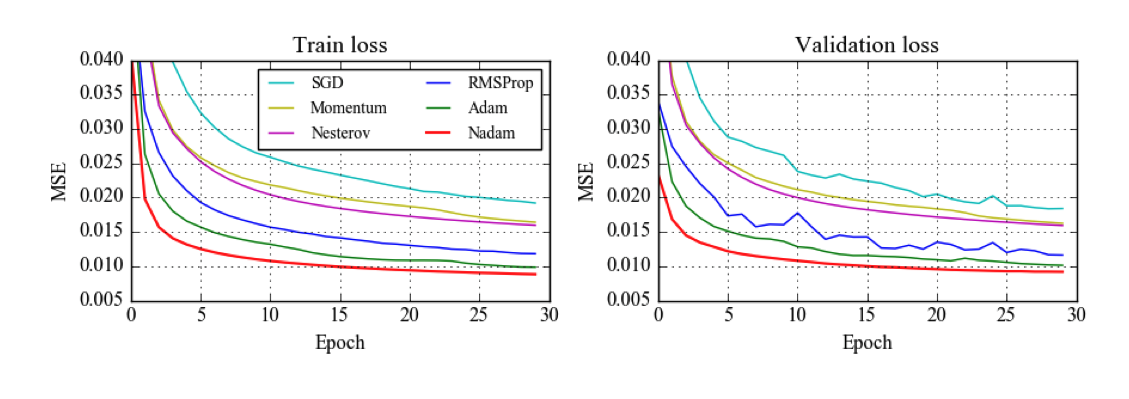
\includegraphics[width=1\linewidth]{../imagens/retropropagacao-gradiente/comparativo-nadam-mnist.png}
    
    \caption[Perda de treinamento e validação com diferentes otimizadores]{%
        Perda de treinamento e validação de diferentes otimizadores no dataset \textit{MNIST}.
        \newline
        \small Fonte: \parencite{NadamMethod}.
    }
    \label{fig:comparativo-nadam-mnist}
\end{figure}
 
Comparando com o \textit{Adam} tradicional, a principal diferença do \textit{NAdam} com esse outro otimizador está justamente relacionada ao decaimento do erro, que é consideravalemente maior, enquanto o \textit{NAdam} já estava se estabilizando com cerca de 10 épocas, o \textit{Adam} parece demorar mais. De fato como apresentado por \textcite{NadamMethod}, o \textit{NAdam} é capaz de acelerar as taxas de convergência do modelo que está sendo treinado.

\medskip
\begin{center}
 * * *
\end{center}
\medskip

\textbf{Algumas Aplicações do NAdam em Otimização de Redes Neurais}
\vspace{1em}

\begin{itemize}
    \item \textbf{Aplicação 1 (Área):}
    \item \textbf{Aplicação 2 (Área):}
    \item \textbf{Aplicação 3 (Área):}
    \item \textbf{Aplicação 4 (Área):}
\end{itemize}

\medskip
\begin{center}
 * * *
\end{center}
\medskip

\subsection{Adam With Decoupled Weight Decay (AdamW)} \index{Otimizadores!Adam With Decoupled Weight Decay (AdamW)}

Uma outra variante do \textit{Adam} tradicional é o \textit{AdamW}. Essa variante foi apresentada no trabalho \textit{Decoupled Weight Decay Regularization} dos pesquisadores \textcite{AdamWMethod}, em que eles propuseram uma forma diferente de corrigir como a relgularização $L^2$, era feita no método original. Para isso, o \textit{AdamW} desacopla o decaimento do peso da atualização principal do do gradiente, e o aplica como um passo separado e final na atualização dos parâmetros \parencite{AdamWMethod}.

Esse algoritmo pode ser visto no psudeocódigo apresentado no bloco \ref{alg:adamw}.

o \textit{AdamW} recebe como entradas a taxa de aprendizado $\eta$, os coeficientes de decaimento $\beta_1$ e $\beta_2$, o fato de decaimento de peso $\lambda$, o vetor contendo os parâmetros iniciais do modelo $\theta_0$, a função de perda a ser otimizada $f(\theta)$ e o parâmetro de estabilidade $\epsilon$. Semelhante ao \textit{Adam}, o \textit{AdamW} começa inicializando os vetores de primeiro $\mathbf{m}_0$ e segundo $\mathbf{v}_0$ momento bem como o passo de tempo $t$.

Feito isso, é iniciado o loop do \textit{AdamW} que irá terminar quando o modelo convergir. Ele começa da mesma forma que os outros otimizadores vistos até agora, incrementa o passo de tempo $t$, e calcula o vetor gradiente da função de perda no passo anterior e o adiciona em $\mathbf{g}_t$. Seguindo adiante são feitas as estimativas dos momentos de forma semelhante ao \textit{Adam}, primeiro calcula-se o primeiro momento $\mathbf{m}_t$ que irá receber a multiplicação do coeficiente de decaimento $\beta_1$ com o momento anterior $\mathbf{m}_{t-1}$ somado a multiplicação do vetor gradiente $\mathbf{g}_t$ com $(1 - \beta_1)$. De forma semelhante é possível calcular o segundo momento $\mathbf{v}_t$ o qual será dado pela multiplicação do coeficiente de decaimento $\beta_2$ com o momento anterior $\mathbf{v}_{t-1}$ soamado ao produto termo da termo do vetor gradiente $\mathbf{g}_t$ com $(1 - \beta_2)$.

O próximo passo do \textit{AdamW} é a correção do viés. Começando com $\mathbf{\hat{m}_t}$ que irá receber a divisão do vetor de momentos $\mathbf{m}_t$ com $(1 - \beta_1^t)$. Já $\mathbf{\hat{v}}_t$ é calculado de forma semelhante, ele irá receber a divisão do vetor de segundo momento $\mathbf{v}_t$ com $(1 - \beta_2^t)$.

A diferença do \textit{AdamW} está nessa próxima parte, o cálculo dos parâmetros $\theta$ para a próxima iteração. Para isso, eles serão dados pela diferença dos parâmetros na iteração anterior $\theta_{t-1}$ com a multiplicação da taxa de aprendizado $\eta$ com a divisão do vetor do primeiro momento já corrigido pela raiz do vetor de segundo momento também já corrigido, isso é então somado ao produto do fator de dacaimento de peso $\lambda$ pelos parâmetros da iteração enterior $\theta_{t-1}$.

\begin{algorithm}[H]
    \caption{Adam com Decaimento de Peso Desacoplado (AdamW)}
    \label{alg:adamw}
    \begin{algorithmic}[1]

    \Require Taxa de aprendizado $\eta$ (ex: 0.001)
    \Require Coeficientes de decaimento $\beta_1, \beta_2$ (ex: 0.9, 0.999)
    \Require Fator de decaimento de peso $\lambda$ (ex: 0.01)
    \Require Vetor de parâmetros inicial $\theta_0$
    \Require Função a ser otimizada $f(\theta)$
    \Require Parâmetro de estabilidade $\epsilon$ (ex: 1e-8)

    \State $\mathbf{m}_0 \leftarrow 0$ \Comment{Inicializar vetor de 1º momento (média)}
    \State $\mathbf{v}_0 \leftarrow 0$ \Comment{Inicializar vetor de 2º momento (variância)}
    \State $t \leftarrow 0$ \Comment{Inicializar passo de tempo}

    \While{não convergir}
        \State $t \leftarrow t + 1$
        \State $\mathbf{g}_t \leftarrow \nabla_{\theta_{t-1}} f(\theta_{t-1})$ \Comment{O gradiente NÃO inclui o termo de decaimento}
        
        % Atualiza estimativas dos momentos (como no Adam)
        \State $\mathbf{m}_t \leftarrow \beta_1 \mathbf{m}_{t-1} + (1 - \beta_1) \mathbf{g}_t$
        \State $\mathbf{v}_t \leftarrow \beta_2 \mathbf{v}_{t-1} + (1 - \beta_2) (\mathbf{g}_t \odot \mathbf{g}_t)$
        
        % Calcula a correção de viés (bias correction)
        \State $\mathbf{\hat{m}}_t \leftarrow \frac{\mathbf{m}_t}{1 - \beta_1^t}$
        \State $\mathbf{\hat{v}}_t \leftarrow \frac{\mathbf{v}_t}{1 - \beta_2^t}$
        
        % Atualiza os parâmetros com decaimento de peso desacoplado
        \State $\theta_t \leftarrow \theta_{t-1} - \eta \left( \frac{\mathbf{\hat{m}}_t}{\sqrt{\mathbf{\hat{v}}_t} + \epsilon} + \lambda \theta_{t-1} \right)$
    \EndWhile

    \State \Return $\theta_t$ \Comment{Parâmetros resultantes}
    \end{algorithmic}
\end{algorithm}

Para compravar a eficácia do desacoplamento de peso, \textcite{AdamWMethod} decidem availiar o \textit{Adam} com reguralização L2 com a nova variante \textit{AdamW} utilizando uma 26 2x64d \textit{ResNet} no \textit{CIFAR-10} medida depois de 100 épocas, além disso, os autores avaliam também o \textit{SGD} e sua variante com peso desacoplado, o \textit{SGDW}, de forma que os resultados podem ser vistos na Figura \ref{fig:comparativo-adamw-cifar-10}.

\begin{figure}[h]
    \centering
    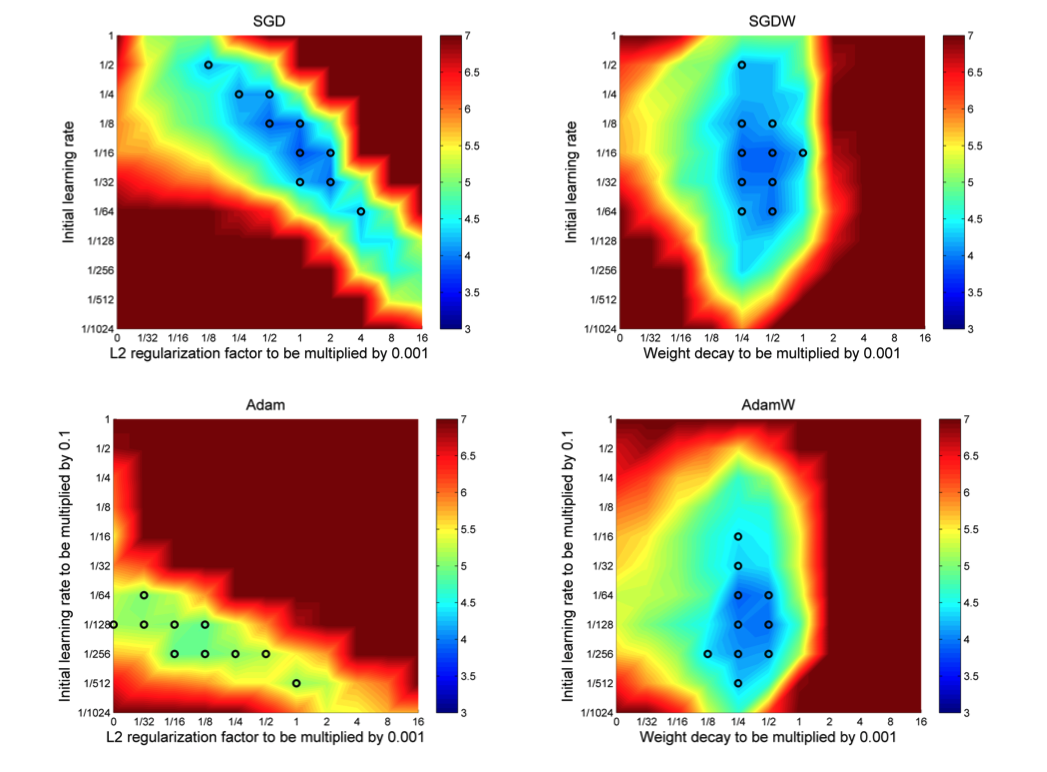
\includegraphics[width=1\linewidth]{../imagens/retropropagacao-gradiente/comparativo-adamw-cifar-10.png}
    
    \caption[Erro de teste Top-1 da ResNet no CIFAR-10]{%
        Erro de teste Top-1 de uma ResNet 26 2x64d no CIFAR-10, medido após 100 épocas. Os métodos propostos SGDW e AdamW (coluna da direita) possuem um espaço de hiperparâmetros mais separável.
        \newline
        \small Fonte: \parencite{AdamWMethod}.
    }
    \label{fig:comparativo-adamw-cifar-10}
\end{figure}

Nessas figuras, o eixo vertical representa a taxa de aprendizado, enquando o eixo horizontal representa a forca de regulariação ou do decaimento do peso. Enquanto isso, as cores indicam o desempenho do momedo, azul e ciano representam um bom desempenho, com baixo erro, enquanto vermelho representa um desemepho pior, com erro mais alto.

Note que ambas as variantes do gradiente estocástico apresentam partes azuis, no \textit{SGD} (a esquerda), a área de de bom desempenho é pequena, além de formar uma faixa diagonal estreita, o que indica que a taxa de aprendizado ideal e a força de reguralização são altamentes dependentes uma da outra. Isso significa que se você escoler um valor da taxa de aprendizado fora dessa faixa, utilizar um modelo com o \textit{SGD} seria difícil para otimizar.

Por outro lado, no \textit{SGDW} a área azul é muito maior além de ser mais vertical, indicando que existe uma ampla variante de taxas de aprendizado que você pode escolher e ainda sim conseguir um modelo bem otimizado. De forma que a escola de um bom decaimento de peso e de uma taxa de aprendizado são mais independentes, e com isso o modelo pode ser mais fácil de otimizar.

Quando comparamos agora as duas variantes do \textit{Adam} vemos um cenário diferente. Note que o resultado do \textit{Adam} é bem ruim, o gráfico é quase todo vermelho, o que mostra que o \textit{Adam} com a reguralização L2 falha em convergir para melhores pontos de mínimo para a maioria das taxas de aprendizado apresentadas.

Agora se analisar o \textit{AdamW} o resultado é bem mais positivo. Assim como o \textit{SGDW} existe uma linha vertical em azul no \textit{AdamW}, o que nos mostra que é possível escolher uma quantidade grande de taxas de aprendizado que permitam ao modelo uma boa convergência, além é claro dela ser mais independente com relação do decaimento de peso.

Assim, utilizar o \textit{AdamW} pode ser uma excelente alternativa caso queira tentar taxas de aprendizado diferentes e ainda sim obter uma boa convergência do modelo. Por exemplo, se quiser você pode escolher uma taxa de aprendizado mais alta, permitindo com que o modelo dê passos mais largos e assim consiga convergir de forma mais rápida. Mas você ainda tem a oportunidade de utilizar taxas de aprendizado menores e provavelmente irá encontrar um ponto de mínimo.

\medskip
\begin{center}
 * * *
\end{center}
\medskip

\textbf{Algumas Aplicações do ADamW em Otimização de Redes Neurais}
\vspace{1em}

\begin{itemize}
    \item \textbf{Aplicação 1 (Área):}
    \item \textbf{Aplicação 2 (Área):}
    \item \textbf{Aplicação 3 (Área):}
    \item \textbf{Aplicação 4 (Área):}
\end{itemize}

\medskip
\begin{center}
 * * *
\end{center}
\medskip

\subsection{Comparativo dos Otimizadores Modernos}

Por fim, com base nos otimizadores vistos nessa seção, assim como foi feito na seção de otimizadores clássicos, é possível fazer uma tabela contendo as suas principais características. Para isso, tem-se então a Tabela \ref{tab:comparativo-otimizadores-modernos}

\begin{table}[htbp]
    \centering
    \begin{threeparttable}
        \caption{Comparativo de otimizadores modernos}
        \label{tab:comparativo-otimizadores-modernos}
        % p{3.2cm} define uma largura fixa para a primeira coluna.
        % As 3 colunas 'X' restantes dividem o espaço que sobra de forma flexível.
        % >{\raggedright\arraybackslash} alinha o texto à esquerda para melhor leitura.
        \begin{tabularx}{\textwidth}{p{3.2cm} *{1}{>{\raggedright\arraybackslash}X}}
            \toprule
            \textbf{Otimizador} & \textbf{Inovação principal} \\
            \midrule
            \textit{AdaGrad} & Faz o uso de múltiplas taxas de aprendizado, garantindo que tanto características comuns, quanto incomuns possam ser aprendidas pelo modelo \\
            \addlinespace
            \textit{RMSProp} & Utiliza um vetor com a média móvel do quadrado dos gradientes que é multiplicado por uma taxa de decaimento, impedindo que o vetor acumulador só cresça. \\
            \addlinespace
            \textit{Adam} & Combina as ideias do \textit{AdaGrad} e \textit{RMSProp} utilizando médias móveis, uma para os gradientes (primeiro momento), e outra para o quadrado dos gradientes (segundo momento). \\
            \addlinespace
            \textit{AdaMax} & Uma variante do Adam baseado na norma infinita. Para isso, ao invés de utilizar a média dos quadrados dos gradientes, ele utiliza o máximo entre o gradiente atual e a média anterior. \\
            \addlinespace
            \textit{Nadam} & Adiciona as ideias do \textit{NAG} no \textit{Adam}, para isso, ele aplica a ideia de \textit{lookahead} ao cálculo da média móvel dos gradientes (primeiro momento). \\
            \textit{AdamW} & Desacopla o decaimento de peso da etapa de atualização do gradiente, aplicando-o diretamete aos pesos, dessa forma, ele consegue corrigir a forma como a regularização do decaimento de peso (L2) é aplicado no \textit{Adam}. \\
            \bottomrule
        \end{tabularx}
        
        \begin{tablenotes}[para]
            \small
            \item[] Fonte: O autor (2025).
        \end{tablenotes}

    \end{threeparttable}
\end{table}

\subsection{Outros Otimizadores}

\textbf{Rectified Adam (RAdam)} \index{Otimizadores!Rectified Adam (RAdam)}

Uma outra variante do \textit{Adam} que também busca melhorar o otimizador original é o \textit{Rectified Adam} ou \textit{RAdam}. Ele surgiu no trabalho \textit{On the Variance of the Adaptive Learning Rate and Beyond} dos autores \textcite{RAdamMethod} como uma atualização do Adam que buscava corrigir um problema identificado com a taxa de aprendizado adaptativa do otimizador: a sua variância é grande problemática nos primeiros estágios; de forma que eles propusaram o \textit{RAdam}, uma variante que introduz um termo para retificar a variância da taxa de aprendizado adpativa.

\textbf{Lion} \index{Otimizadores!Lion}

\section{Comparativo de Desempenho: Otimizadores}

% ===================================================================
% Método de Newton
% ===================================================================

\section{O Método de Newton: Indo Além do Gradiente}

O método do gradiente se enquadra no tipo de \textbf{método de primeira ordem}, pois faz o uso de apenas derivadas de primeira ordem na sua implementação. Existem métodos que vão além das derivadas de primeira ordem buscando soluções que fazem uso de \textbf{derivadas de segunda ordem}. Um desses métodos é o \textbf{método de Newton}.

Essa técnica foi inicialmente proposta por Isaac Newton nos trabalhos “\textit{De analysi per aequationes numero terminorum infinitas}” em 1669 e “\textit{De metodis fluxionum et serierum infinitarum}” escrito em 1671. Entretanto, mais tarde Joseph Raphson apresentou uma versão aprimorada em seu livro “\textit{Aequationum Universalis}” em 1690. Devido às contribuições de ambos os matemáticos, essa técnica também é conhecida como método de Newton-Raphson.

\subsection{Conceitos iniciais: Matrizes Jacobianas e Hessianas}

Como dito anteriormente, o método de Newton faz uso de derivadas de segunda ordem em sua fórmula. Nisso, surgem dois conceitos que devem ser explicados para entendermos melhor esse método: as matrizes jacobianas e hessianas.

Chamamos de \textbf{matriz jacobiana} a matriz que contém todos as derivadas parciais de uma função de $n$ variáveis $f(x, y, ..., n)$. Com base nas derivadas de primeira ordem, podemos ter uma melhor noção de como a função cresce ou decresce em intervalos do eixo.

    \begin{equation}
        \large J_f(x,y,...,n) =
        \begin{bmatrix}
        \frac{\partial F_1}{\partial x} & \frac{\partial F_1}{\partial y} & \cdots & \frac{\partial F_1}{\partial n} \\
        \frac{\partial F_2}{\partial x} & \frac{\partial F_2}{\partial y} & \cdots & \frac{\partial F_2}{\partial n} \\
        \vdots & \vdots & \ddots & \vdots \\
        \frac{\partial F_m}{\partial x} & \frac{\partial F_m}{\partial y} & \cdots & \frac{\partial F_m}{\partial n}
        \end{bmatrix}
    \end{equation}

Já a \textbf{matriz hessiana} é uma matriz que contém todas as derivadas de segunda ordem da função $f(x, y, ..., n)$. Essas derivadas nos dão informações sobre a curvatura a função.

    \begin{equation}
        \large H_f(x,y,...,n) =
        \begin{bmatrix}
        \frac{\partial^2 f}{\partial x^2} & \frac{\partial^2 f}{\partial x\partial y} & \cdots & \frac{\partial^2 f}{\partial x \partial n} \\
        \frac{\partial^2 f}{\partial y \partial x} & \frac{\partial^2 f}{\partial y^2} & \cdots & \frac{\partial^2 f}{\partial y \partial n} \\
        \vdots & \vdots & \ddots & \vdots \\
        \frac{\partial^2 f}{\partial n \partial x} & \frac{\partial^2 f}{\partial n \partial y} & \cdots & \frac{\partial^2 f}{\partial n^2}
        \end{bmatrix}
    \end{equation}

Assim, essas matrizes, por nos mostrarem como a função varia, podem ser muito úteis para nos auxiliar a encontrar pontos mínimos, máximos e de sela da função e assim otimizá-la.

Com isso, podemos entender o método de newton.

\subsection{O Método}

O método de Newton é baseado na expansão de uma função $f(x)$ em uma \textbf{série de Taylor de segunda ordem} em torno de um ponto $x(0)$. Com essa aproximação, podemos encontrar de forma mais rápida pontos críticos da função.

    \begin{equation}
         f(\mathbf{x}) \approx f(\mathbf{x}_0) + \nabla f(\mathbf{x}_0)^T (\mathbf{x} - \mathbf{x}_0) + \frac{1}{2} (\mathbf{x} - \mathbf{x}_0)^T H_f(\mathbf{x}_0) (\mathbf{x} - \mathbf{x}_0)
    \end{equation}

    \begin{equation}
         x' = x - H_f(x)^{-1} \nabla f(x)
    \end{equation}

Quando estamos trabalhando com uma função que pode ser aproximada por uma função quadrática no ponto analisado, o método de Newton pode nos retornar o resultado de forma mais rápida que o método do gradiente. Contudo, se isso não for o caso, ele levará mais iterações para encontrar um ponto crítico e assim convergir.

Por mais que possa ser mais rápido que o método do gradiente em algumas situações, o método de Newton não é perfeito. Se estivermos próximo tanto de ponto de sela quanto de um ponto de mínimo, o método de Newton pode fornecer direções equivocadas e levar para o ponto de sela ao invés do ponto de mínimo. Assim, a não será encontrado um valor ideal para otimizar aquela função de custo.

Além disso, pelo fato do método de Newton envolver o cálculo das derivadas de segunda ordem da função de custo, pois, diferente do método do gradiente que calcula somente as derivadas de primeira ordem, no método de Newton-Raphson são calculadas também as derivadas parciais de segunda ordem para a matriz hessiana.

 Esse custo de poder de processamento será proporcional a quantidade de variáveis que a função de custo recebe, se $f$ for uma função de várias variáveis, pode ser inviável o uso do método de newton devido à maior quantidade de cálculos envolvidos.

Portanto ao criar uma rede neural devemos escolher com sabedoria qual método de otimização devemos usar. O método do gradiente pode ser eficiente para minimizar uma função de custo de uma rede neural, mas em casos que essa convergência seja lenta, o método de Newton-Raphson pode ser uma melhor alternativa.

\textbf{Implementação em Python}

